\begin{enumerate}
\def\labelenumi{\arabic{enumi})}
\setcounter{enumi}{22}
\tightlist
\item
  设 \((\mathrm{W},\mathrm{S})\) 是一个 Coxeter 系统，\(k\) 是交换环。假设对于所有 \(s\in S\) ，给定 \(\lambda_{s}\) 中的两个元素 \(\mu_s\) 和 \(k\)，使得当 \(\lambda_{s} = \lambda_{s'}\) 与 \(\mu_{s} = \mu_{s'}\) 在 W 中共轭时，\(s\) 且 \(s'\)。置 \(\mathbf{E} = k^{(\mathbf{W})}\)，并令 \(\{e_w\}\) 为 E 的标准基。
\end{enumerate}

\begin{enumerate}
\def\labelenumi{\alph{enumi})}
\tightlist
\item
  证明 \(E\) 有唯一的代数结构，使得对于 \(s \in S\) 和 \(w \in W\)，
\end{enumerate}

\[
e _ {s}. e _ {w} = \left\{ \begin{array}{l l} e _ {s w} & \text {if} l (s w) > l (w) \\ \lambda_ {s} e _ {w} + \mu_ {s} e _ {s w} & \text {if} l (s w) <   l (w) \end{array} \right.
\]

(引入 E 的端同态 \(P_{s}\)，其由上述公式定义，其中以 \(e_{s}.e_{w}\) 替换 \(\mathrm{P}_{s}(w)\)；再引入端同态 \(Q_{s}=jP_{s}j^{-1}\)，其中 j 表示由 \(j(e_{w})=e_{w^{-1}}\) 定义的 E 的自同态；注意到条件 \(P_{s}Q_{t}=Q_{t}P_{s}\) 和 \(s,t\in S\) 蕴含 sw=wt，从而证明对于 \(l(swt)=l(w)\) 有 \(l(sw)=l(wt)\)；然后仿照习题 3 c) 论证。赋予此代数结构的模 E 记为 \(\mathrm{E}_{k}((\lambda_{s}),(\mu_{s}))\)。证明 \(\mathrm{E}((0),(1))\) 是 W 的群代数 k{[}W{]}（《代数》，第 III 章，§2，第 6 号）。

b) 证明生成元族 \((e_s)_{s\in S}\) 以及关系

\[
e _ {s} ^ {2} = \lambda_ {s} e _ {s} + \mu_ {s} \mathrm{for} s \in S
\]

\((e_s e_t)^r = (e_t e_s)^r\) 其中 \(s, t \in S\) 且 \(st\) 的有限偶阶为 \(2r\) \((e_s e_t)^r e_s = (e_t e_s)^r e_t\) 其中 \(s, t \in S\) 且 \(st\) 的有限奇阶为 \(2r + 1\)

给出代数 \(\mathbf{E}\) 的一个表示（仿照§1 第 6 号定理 1 的证明）。

\begin{enumerate}
\def\labelenumi{\arabic{enumi})}
\setcounter{enumi}{23}
\tightlist
\item
  设 G 是群，B 是 G 的一个 Tits 子群（习题 3，以下沿用其中的记号）。假设对于所有 \(s \in S\)，双陪集 \(C(s)\) 是关于 B 的有限个左陪集（其数目为 \(q_{s}\)）的并。沿用习题 22 的记号，并对所有 \(a_{w} = a_{\mathrm{C}(w)}\) 置 \(w \in W\)。
\end{enumerate}

\begin{enumerate}
\def\labelenumi{\alph{enumi})}
\item
  证明习题 22 的条件 (i) 和 (ii) 得到满足。因此可以谈论 Hecke 代数 \(\mathrm{H}_k(\mathbf{G},\mathbf{B})\)（\(k\) 为交换环），其中 \((a_w)_{w\in \mathbb{W}}\) 是一组基。
\item
  设 \(s \in S\) 且 \(w \in W\)。证明 \(a_s * a_s = (q_s - 1)a_s + q_s\)；证明若 \(l(sw) > l(w)\)，则 \(a_s * a_w = a_{sw}\)。
\item
  证明从与 Coxeter 系统 (W,S) 相关的代数 \(\mathrm{E}_{k}((q_{s}-1),(q_{s}))\)（习题 23）到 \(\mathrm{H}_{k}(\mathrm{G},\mathrm{B})\) 的线性映射是代数同构，其中对所有 \(e_{w}\) 将 \(a_{w}\) 送到 \(w \in W\)。
\end{enumerate}

\begin{enumerate}
\def\labelenumi{\arabic{enumi})}
\setcounter{enumi}{24}
\tightlist
\item
  沿用习题 8 的记号。另假设对于所有 \(s \in S\)，指数 \(q_s\) 是 \(B \cap gBg^{-1}\) 在 \(B\) 中的指数，并且对所有 \(g \in BsB\) 该指数是有限的。
\end{enumerate}

\begin{enumerate}
\def\labelenumi{\alph{enumi})}
\item
  证明对 \((\tilde{\mathbf{G}},\mathbf{B})\) 满足习题 22 的条件 (i) 和 (ii)。
\item
  证明对于所有 \(\gamma \in \Gamma\)，映射 \(x \mapsto \gamma x \gamma^{-1}\) 定义 Hecke 代数 \(\sigma\) 的一个自同态 \(\mathrm{H}_k(\mathrm{G}, \mathrm{B})\)，且 \(\sigma\) 只依赖于 \(\omega\) 在 \(\gamma\) 中的类 \(\Omega = \Gamma / (\Gamma \cap \mathrm{B})\)。
\item
  令 \(k[\Omega]\) 为 \(\Omega\) 的群代数，\((e_{\omega})\) 为其标准基。证明从 \(j\) 到 \(k[\Omega] \otimes_k \mathrm{H}_k(\mathbf{G}, \mathbf{B})\) 的线性映射 \(\mathrm{H}_k(\tilde{\mathrm{G}}, \mathrm{B})\) 由 \(j(e_{\omega} \otimes a_{\mathrm{B}w\mathrm{B}}) = a_{\mathrm{B}\omega w\mathrm{B}}\) 定义（采用习题 22 的记号），对于 \(\omega \in \Omega\) 和 \(w \in W\)，是双射，并且
\end{enumerate}

\[
j ^ {- 1} (j (e _ {\omega} \otimes x) j (e _ {w ^ {\prime}} \otimes y)) = e _ {w w ^ {\prime}} \otimes \sigma_ {\omega} (x) y
\]

其中 \(\omega, \omega' \in \Omega\)，且 \(x, y \in \mathrm{H}_k(\mathrm{G}, \mathrm{B})\)。

\begin{enumerate}
\def\labelenumi{\arabic{enumi})}
\setcounter{enumi}{25}
\tightlist
\item
  若 E 是交换域 k 上有限秩的绝对半单代数，则 E 的数值不变量是整数序列 \((n_{1},\ldots,n_{r})\)，满足 \(n_{1}\geqslant\cdots\geqslant n_{r}>0\)，并且对于 k 的任意代数闭包 \(\bar{k}\otimes_{k}E\)，\(\bar{k}\) 同构于 \(\prod M_{n_{i}}(\bar{k})\)。
\end{enumerate}

设 V 是整环，K 是其分式域，\(\varphi\) 是从 V 到交换域 k 的同态，E 是 V-代数。假设 E 是有限秩自由 V-模，并置 \(E_{0} = E \otimes_{V} k\) 和 \(E_{1} = E \otimes_{V} K\)。

\begin{enumerate}
\def\labelenumi{\alph{enumi})}
\item
  假设 \((x,y)\mapsto\mathrm{Tr}_{\mathbb{E}_{0}/k}(xy)\) 上的双线性型 \(E_{0}\) 非退化。证明 \(E_{0}\) 和 \(E_{1}\) 都是绝对半单的（参见《代数》，第 IX 章，§2，习题 1）。
\item
  假设 \(E_{0}\) 和 \(E_{1}\) 分别是 k 和 K 上的绝对半单代数。证明 \(E_{0}\) 和 \(E_{1}\) 具有相同的数值不变量（化归到 k 和 K 都代数闭的情形）；令 \((e_{i})\) 为 E 在 V 上的一组基，令 \((\mathbf{X}_i)\) 为不定元。证明 \(\sum_{i}\mathbf{X}_{i}e_{i}\) 中元素 \(\mathrm{E}_1\otimes_{\mathrm{K}}\mathrm{K}[(\mathrm{X}_i)]\) 的特征多项式（分别地，\(\mathrm{E}_0\otimes_kk[(\mathrm{X}_i)]\) 中相应元素的特征多项式）具有形式 \(\mathrm{P} = \prod_j\mathrm{P}_j^{n_j}\)（分别为 \(\mathrm{Q} = \prod_k\mathrm{Q}_k^{m_k}\)），其中 \((n_1,\ldots ,n_r)\)（分别为 \((m_1,\dots ,m_s))\) 是 \(\mathrm{E}_1\)（分别为 \(\mathrm{E}_0\)）的数值不变量，且 \(\deg (\mathrm{P}_j) = n_j\)（分别为 \(\deg (\mathrm{Q}_k) = m_k\)）。证明 \(\mathrm{P}_j\in \mathrm{V}[(\mathrm{X}_i)]\) 且 \(\mathrm{Q} = \varphi (\mathrm{P})\)。推知存在整数 \(c_{jk}\geqslant 0\)，使得
\end{enumerate}

\[
m _ {k} = \sum_ {j} c _ {j k} n _ {j}, \text { and } n _ {j} = \sum_ {k} c _ {j k} m _ {k}.
\]

*27) 设 \((\mathrm{G},\mathrm{B},\mathrm{N},\mathrm{S})\) 是一个 Tits 系统，且 \(k\) 是交换域。假设 G 是有限群，且 \(k\) 的特征既不整除 G 的阶，也不整除 Weyl 群 \(\mathrm{W} = \mathrm{N} / (\mathrm{B}\cap \mathrm{N})\) 的阶。证明代数 \(\mathrm{H}_k(\mathrm{G},\mathrm{B})\)（习题 22）和 \(k[\mathrm{W}]\) 都是绝对半单的并具有相同的数值不变量，因而当 \(k\) 代数闭时二者同构（令 \(q_{s}\) 为 \(\mathrm{B}\cap g\mathrm{Bg}^{-1}\)、\(g\in \mathrm{BsB}\) 时 \(s\in S\) 在 B 中的指数）。考虑按照习题 23 从 Coxeter 系统 (W,S) 和多项式环 \(\mathrm{E}_{k[\mathrm{X}]}((\mathrm{X}(q_s - 1)),(1 + \mathrm{X}(q_s - 1)))\) 构造的代数 \(k[\mathrm{X}]\)，并使用习题 26 a) 和 b)，注意根据 Maschke 定理（第 V 章，附录），双线性型 \(\mathrm{Tr}_{k[\mathrm{W}] / k}(xy)\) 是非退化的）。*

\begin{enumerate}
\def\labelenumi{\arabic{enumi})}
\setcounter{enumi}{27}
\item
  设 G 是群，M 是 G 的极大子群，U 是 M 的正规子群，满足第 7 号的条件 (R)。假设 G 等于其换位子群，由 U 的共轭子群之并生成，且 M 的共轭子群之交化为单位元。证明 G 是单群。（考虑 G 的一个不同于 \{1\} 的正规子群 N；证明 G = N.M，进而证明 G = N.U。）
\item
  设 H 是非阿贝尔单群。设 \(\theta\) 是 H 的一个阶为素数 p 的自同构，U 是由 \(\theta\) 对应的 Z/pZ 与 H 的半直积。证明若 \(\theta\) 不是内自同构，则 U 的正规子群只有 \(\{1\}\)、H 和 U。推知 U 不可解，但满足第 7 号的条件 (R)。应用此结论证明对称群 \(S_{n}\) 满足条件 (R)。
\end{enumerate}

\chapter{由反射生成的群}

\section{超平面、室与面片}

在本节中，E 表示有限维为 d 的实仿射空间，T 表示 E 的平移空间（参见《代数》，第 II 章，§9）。若 a 和 b 是 E 的两个点，则 {[}ab{]}（分别地，{]}ab{[}，以及 {]}ab{]}）表示端点为 a、b 的闭线段（分别为开线段，以及在 a 处开而在 b 处闭的线段）。T 赋予其唯一的 Hausdorff 拓扑向量空间拓扑，参见《拓扑向量空间》，第 I 章，§2，第 3 号；它同构于 \(R^{d}\)。E 赋予唯一的拓扑，使得对于所有 \(e \in E\)，从 T 到 E 的映射 \(t \mapsto e + t\) 是同胚。

记 H 为 E 的一个局部有限超平面集（《一般拓扑》，第 I 章，§1，第 5 号）。

\subsection{记号}

设 H 是 E 的一个超平面。回忆 E-H 有两个连通分支，称为由 H 界定的开半空间。它们的闭包称为由 H 界定的闭半空间。设 \(x, y \in E\)。如果 x 和 y 包含在由 H 界定的同一个开半空间内，或者等价地说，端点为 x 和 y 的闭线段不与 H 相交，则称 x 和 y 严格位于 H 的同侧；如果 x 属于由 H 界定的一个开半空间而 y 属于另一个，则称 x 和 y 位于 H 的相反两侧。若 \(x \in E\) 且 \(t \in T\)，如果对于所有 \(h + t\)，x 和 \(h \in H\) 严格位于 H 的同侧，则称 x 和 t 严格位于 H 的同侧。

设 A 是 E 的非空连通子集。对于 E 中不与 A 相交的任意超平面 H，用 \(D_{H}(A)\) 表示包含 A 的、由 H 界定的唯一开半空间。若 N 是 E 的一个超平面集，且其中没有一个与 A 相交，置

\[
D _ {\mathfrak {N}} (A) = \bigcap_ {H \in \mathfrak {N}} D _ {H} (A).\tag{1}
\]

如果 \(\mathrm{A}\) 由单点 \(a\) 组成，则我们用 \(\mathrm{D_H}(a)\) 和 \(\mathrm{D}_{\mathfrak{N}}(a)\) 代替 \(\mathrm{D_H}(\{a\})\) 和 \(\mathrm{D}_{\mathfrak{N}}(\{a\})\)。

\subsection{面片}

不属于超平面集 H 中任何超平面的 E 中点集是开集，因为 H 是局部有限的。更精确地，有如下结果：

命题 1. 设 a 是 E 的一点。存在 a 的一个连通开邻域，它不与属于 H 且不经过 a 的任何超平面相交。此外，属于 H 且经过 a 的超平面只有有限多个。

满足 \(H \in H\) 且 \(a \notin H\) 的超平面 H 所成的集合 N 是局部有限的，因为它包含于 H 中。因此，不属于 N 中任何超平面的 E 中点集 U 是开集。由于 \(a \in U\)，存在包含于 U 的 a 的连通开邻域。命题的其余部分显然。

给定两点 \(x\) 和 \(y\)，它们属于 \(\mathbf{E}\)，用 \(\mathrm{R}\{x,y\}\) 表示关系

“对于任意超平面 \(H \in H\)，或者 \(x \in H\) 且 \(y \in H\)，或者 x 和 y 严格位于 H 的同侧。”

显然，R 是 E 上的等价关系。

定义 1. 相对于 \(\mathfrak{H}\) 的 E 的一个面片，是上述等价关系的一个等价类。

命题 2. 面片集是局部有限的。

这显然是因为 \(\mathfrak{H}\) 是局部有限的。

设 F 是一个面片，\(a\) 是 F 的一点。超平面 \(H \in H\) 包含 F 当且仅当 \(a \in H\)；因此这些超平面所成的集合 F 是有限的；它们的交是 E 的一个仿射子空间 L，我们称其为 F 的仿射支撑；L 的维数称为 F 的维数。

若 \(\mathfrak{N}\) 是超平面 \(H\in \mathfrak{H}\) 中不包含 \(F\) 的那些超平面所成的集合，则

\[
F = L \cap \bigcap_ {H \in \mathfrak {N}} D _ {H} (a).\tag{2}
\]

我们将证明 F 的闭包由下式给出：

\[
\overline {{F}} = L \cap \bigcap_ {H \in \mathfrak {N}} \overline {{D _ {H} (a)}}.\tag{3}
\]

显然，右端包含左端。反之，设 \(x \in L \cap \bigcap_{H \in \mathfrak{N}} \overline{\mathrm{D}_H(a)}\)。端点为 \(a\) 和 \(x\) 的开线段包含于 \(L\) 以及每个 \(D_H(a)\)（对于 \(H \in \mathfrak{N}\)）中，因而包含于 \(F\) 中。于是 \(x\) 属于 \(F\) 的闭包，公式得证。

命题 3. 设 F 是一个面片，L 是其仿射支撑。

\begin{enumerate}
\def\labelenumi{(\roman{enumi})}
\item
  集合 \(\mathbf{F}\) 是 \(\mathbf{L}\) 的仿射子空间 \(\mathbf{E}\) 的凸开子集。
\item
  \(\mathbf{F}\) 的闭包是 \(\mathbf{F}\) 与维数严格小于 \(\mathbf{F}\) 的面片之并。
\item
  在拓扑空间 L 中，集合 F 是其闭包的内部。
\end{enumerate}

由于每个开半空间和每个超平面都是 E 的凸子集，公式 (2) 表明 F 是一族凸子集的交，因而是凸的。另一方面，设 a 属于 F，取 E 中 a 的一个凸开邻域 U，使其不与集合 N 中的任何超平面相交，其中 N 由满足 \(H \in H\) 且 \(a \notin H\) 的 H 组成。于是对于任意 \(H \in N\)，有 \(U \subset D_{H}(a)\)，从而 \(L \cap U \subset F\)，所以 F 在拓扑空间 L 中是开的。

设 \(b\) 是 \(\overline{F} - F\) 中属于一个面片 \(F'\) 的点，令 \(\mathfrak{N}'\) 为经过 \(H \in \mathfrak{N}\) 的、属于 \(b\) 的超平面所成的集合；置 \(\mathfrak{N}'' = \mathfrak{N} - \mathfrak{N}'\)。对于 \(H\) 中的任意 \(\mathfrak{N}''\)，有 \(b \notin H\) 且 \(b \in \overline{D_H(a)}\)，因而 \(b \in D_H(a)\) 且 \(D_H(b) = D_H(a)\)；由面片的定义，故有

\[
F ^ {\prime} = L \cap \bigcap_ {H \in \mathfrak {N} ^ {\prime}} H \cap \bigcap_ {H \in \mathfrak {N} ^ {\prime \prime}} D _ {H} (a),\tag{4}
\]

而 (3) 蕴含

\[
\overline {{\mathbf {F}}} = \mathbf {L} \cap \bigcap_ {\mathsf {H} \in \mathfrak {N} ^ {\prime}} \overline {{\mathsf {D} _ {\mathsf {H}} (a)}} \cap \bigcap_ {\mathsf {H} \in \mathfrak {N} ^ {\prime \prime}} \overline {{\mathsf {D} _ {\mathsf {H}} (a)}},\tag{5}
\]

于是 \(\mathbf{F}' \subset \overline{\mathbf{F}}\)。不能有 \(\mathfrak{N}' = \varnothing\)，因为由 (2) 和 (4) 这将推出 \(\mathbf{F} = \mathbf{F}'\)，这与假设 \(b \notin \mathbf{F}\) 且 \(b \in \mathbf{F}'\) 矛盾。\(\mathbf{F}'\) 的支撑是集合 \(\mathbf{L}' = \mathbf{L} \cap \bigcap_{\mathbf{H} \in \mathfrak{N}'} \mathbf{H}\)；我们有 \(a \in \mathbf{L}\)，但对于 \(a \notin \mathbf{H}\) 中的 \(\mathbf{H}\)，有 \(\mathfrak{N}'\)，所以 \(\mathbf{L}' \neq \mathbf{L}\)，最终 \(\dim \mathbf{L}' < \dim \mathbf{L}\)，即 \(\dim \mathbf{F}' < \dim \mathbf{F}\)。这证明了 (ii)。

设 H 属于 \(N'\)，令 D 为由 H 界定且不同于 \(D_{\mathrm{H}}(a)\) 的开半空间；有 \(b \in H \cap L\)，并且立即可见，\(D \cap L\) 是 L 中由 L 的超平面 \(H \cap L\) 界定的半空间；因此，L 中 b 的每个邻域都与 \(D \cap L\) 相交，而由 (3)，\(D \cap L\) 与 \(\overline{F}\) 不相交，于是可见 \(\overline{F} - F\) 中的点 b 不可能是拓扑空间 L 中 \(\overline{F}\) 的内部点。由于 F 在 L 中开，得到 (iii)。证毕。

推论. 设 F 和 \(F'\) 是两个面片。若 \(\overline{F} = \overline{F'}\)，则面片 F 和 \(F'\) 相等。

这由 (iii) 得出。

命题 4. 设 F 是一个面片，L 是 E 的一个仿射子空间，且它是属于 H 的超平面的交：记 N 为不包含 L 的超平面 \(H \in H\) 所成的集合。下列条件等价：

\begin{enumerate}
\def\labelenumi{(\roman{enumi})}
\item
存在面片 \(\mathbf{F}'\)，它的支撑为 L 且与 \(\overline{\mathbf{F}}\) 相交。
\item
存在面片 \(\mathbf{F}'\)，其支撑为 \(\mathbf{L}\) 且包含于 \(\overline{\mathbf{F}}\)。
\item
存在点 \(x\) 属于 \(\mathbf{L} \cap \overline{\mathbf{F}}\)，但不属于 \(\mathfrak{N}\) 中的任何超平面。
\end{enumerate}

若这些条件满足，\(\mathrm{L} \cap \mathrm{D}_{\mathfrak{M}}(\mathrm{F})\) 是支撑为 \(\mathrm{L}\) 且包含于 \(\overline{\mathbf{F}}\) 的唯一面片。

\begin{enumerate}
\def\labelenumi{(\roman{enumi})}
\item
\(\Longrightarrow\) (ii)：由于 \(\overline{\mathbf{F}}\) 是面片的并（命题 3，(ii)），每个与 \(\overline{\mathbf{F}}\) 相交的面片都与包含于 \(\overline{\mathbf{F}}\) 的一个面片相交，因而与该面片相等。
\item
\(\Longrightarrow\) (iii)：对每个 \(x\) 属于 \(F'\)，(iii) 成立，因为 \(\mathfrak{H}\) 中包含 \(x\) 的每个超平面都包含 \(F'\)，因而也包含 \(L\)。
\item
\(\Longrightarrow\) (i)：设 \(x\) 是满足 (iii) 的一点，并令 \(\mathbf{F}'\) 为包含 \(x\) 的面片；显然，\(\mathbf{F}'\) 与 \(\overline{\mathbf{F}}\) 相交。令 \(\mathrm{H} \in \mathfrak{H}\)；则 \(x \notin \mathrm{H}\) 当 \(\mathrm{H} \in \mathfrak{N}\) 时成立，而显然 \(x \in \mathrm{H}\) 当 \(\mathrm{H} \notin \mathfrak{N}\) 时成立；因此，\(\mathbf{F}'\) 的支撑是 \(\mathfrak{H} - \mathfrak{N}\) 中超平面的交，并且等于 \(\mathrm{L}\)。
\end{enumerate}

最后，设 \(F'\) 是一个支撑为 L 且包含于 \(\overline{F}\) 的面片，x 是 \(F'\) 的一点；由于没有 \(N \subset H\) 中的超平面经过 x，命题 1 表明存在 x 的一个凸开邻域 U，使其不与 N 中任何超平面相交。由于 x 属于 F 的闭包，\(U \cap F \neq \varnothing\)；现在 N 是不包含 \(H \in H\) 的超平面 \(F'\) 所成的集合，对于 N 中的所有 H，有 \(D_{H}(x) = D_{H}(U) = D_{H}(U \cap F) = D_{H}(F)\)，由公式 (2) 得

\[
\mathrm{F} ^ {\prime} = \mathrm{L} \cap \mathrm{D} _ {\mathfrak {N}} (\mathrm{F}). \quad \text { Q.E.D. }
\]

\subsection{室}

定义 2. 相对于 H 的 E 的一个室（如果关于 H 没有歧义，也简称为室）是相对于 H 的 E 的一个不包含于属于 H 的任何超平面的面片。

设 U 是 E 中由不属于 H 的任何超平面的点组成的开集；由于 H 中的超平面若与某个面片相交就必须包含该面片，室就是包含于 U 的面片；由命题 3 (i)，每个室都是 E 的凸（因而连通）开子集；由于室构成 U 的一个划分，它们恰好是 U 的连通分支。U 的每个凸子集 A 都是连通的，因而包含于一个室中；若 A 非空，该室是唯一的。显然，室就是支撑为 E 的面片，而命题 3 (iii) 表明每个室都是其闭包的内部。最后，设 C 是一个室，A 是 C 的非空子集；公式 (2) 和 (3) 蕴含

\[
C = \bigcap_ {H \in \mathfrak {H}} D _ {H} (A) = D _ {\mathfrak {H}} (A), \quad \overline {{C}} = \bigcap_ {H \in \mathfrak {H}} \overline {{D _ {H} (A)}}\tag{6}
\]

因为对于所有 \(D_{\mathrm{H}}(\mathbf{A}) = D_{\mathrm{H}}(a)\)，有 \(a \in A\)。

命题 5. 设 C 是 E 的非空子集。假设 \(\mathfrak{H}'\) 存在一个子集 \(\mathfrak{H}\)，具有下列性质：

\begin{enumerate}
\def\labelenumi{\alph{enumi})}
\item
  对于任意 \(\mathrm{H} \in \mathfrak{H}'\)，存在由 \(\mathrm{D}_{\mathrm{H}}\) 界定的开半空间 \(\mathrm{H}\)，使得 \(\mathrm{C} = \bigcap_{\mathrm{H} \in \mathfrak{H}'} \mathrm{D}_{\mathrm{H}}\)。
\item
  集合 C 不与属于 \(\mathfrak{H} - \mathfrak{H}'\) 的任何超平面相交。
\end{enumerate}

在这些条件下，C 是 \(\mathfrak{H}\) 在 E 中定义的一个室，并且对于所有 \(\mathrm{D_H} = \mathrm{D_H(C)}\)，\(\mathrm{H} \in \mathfrak{H}\)。

性质 a) 和 b) 表明 C 是 U 的凸子集；因此存在一个室 \(C'\)，使 \(C \subset C'\)。由于 \(C \subset D_{H}\)，对 \(D_{H} = D_{H}(C)\) 中的所有 H，有 \(H'\)，从而 \(C = D_{H'}(C) \supset D_{H}(C)\)，因为 \(H' \subset H\)；由 (6)，有 \(D_{H}(C) = C'\)，因而 \(C \supset C'\)。最终 \(C = C'\)。

命题 6. E 的每一点都至少属于一个室的闭包。

如果 E 退化为单点，这是显然的。否则，设 \(a \in E\)，令 \(H_{1}, \ldots, H_{m}\) 为 H 中包含 a 的超平面。由于 H 局部有限，存在 a 的一个邻域 V，它不与 H 中除 \(H_{1}, \ldots, H_{m}\) 之外的任何超平面相交。令 D 为经过 a 且不包含于任何 \(H_{i}\) 的直线；若 \(x \in D\)、\(x \neq a\)，且 x 充分接近 a，则开线段 \(|ax|\) 包含于 V 中，且不与任何 \(H_{i}\) 相交。于是 \(|ax| \subset U\)；由于 \(|ax|\) 连通，它包含于一个室 C 中，因而 \(a \in \overline{C}\)。

命题 7. 设 L 是 E 的一个仿射子空间，\(\Omega\) 是 L 的一个非空开子集。

\begin{enumerate}
\def\labelenumi{(\roman{enumi})}
\item
  \(a\) 中存在一点 \(\Omega\)，不属于 \(\mathfrak{H}\) 中不包含 \(L\) 的任何超平面。
\item
  如果 \(\mathrm{L}\) 是超平面且 \(\mathrm{L} \notin \mathfrak{H}\)，则存在一个与 \(\Omega\) 相交的室。
\item
  如果 \(\mathrm{L}\) 是超平面且 \(\mathrm{L} \in \mathfrak{H}\)，则 \(a\) 中存在一点 \(\Omega\)，不属于 \(\mathrm{H} \neq \mathrm{L}\) 中任何超平面 \(\mathfrak{H}\)。
\end{enumerate}

记 N 为满足 \(H \in H\) 且 \(L \notin H\) 的超平面 H 所成的集合，记 L 为仿射空间 L 中形如 \(L \cap H\)（其中 \(H \in N\)）的超平面所成的集合。显然，L 是 L 中的局部有限超平面集，而命题 6 表明 \(\Omega\) 与 L 在 L 中定义的一个室 \(\Gamma\) 相交。若 a 是 \(\Gamma \cap \Omega\) 中的一点，则对所有 \(a \notin H\) 有 \(H \in N\)，从而得到 (i)。

现在假设 L 是超平面；于是包含 L 的任意超平面都等于 L，因此可分为两种情形：

\begin{enumerate}
\def\labelenumi{\alph{enumi})}
\item
  \(\mathbf{L} \notin \mathfrak{H}\)：则 \(\mathfrak{N} = \mathfrak{H}\)，并且对于所有 \(a \notin \mathbf{H}\) 有 \(\mathbf{H} \in \mathfrak{H}\)；因此 \(a\) 属于 \(\mathfrak{H}\) 在 \(\mathbf{E}\) 中定义的一个室，从而得到 (ii)。
\item
  \(\mathrm{L} \in \mathfrak{H}\)：则 \(\mathfrak{N} = \mathfrak{H} - \{\mathrm{L}\}\)，从而得到 (iii)。
\end{enumerate}

\subsection{墙与面}

定义 3. 设 C 是 E 的一个室。C 的一个面是包含于 C 的闭包且支撑为超平面的面片。C 的一面墙是某个 C 的面的支撑超平面。

C 的每一面墙都属于 H。命题 4 表明，超平面 \(L \in H\) 是 C 的一面墙，当且仅当 \(C \neq D_{\mathfrak{H} - \{L\}}(C)\)。此外，C 的每一面墙都是 C 的唯一一个面的支撑。

命题 8. 属于 H 的每个超平面 H 至少是一个室的一面墙。

由命题 7 (iii)，\(a\) 中存在一点 \(\mathbf{H}\)，不属于 \(\mathbf{H}' \neq \mathbf{H}\) 中任何超平面 \(\mathfrak{H}\)；由命题 6，存在一个室 \(\mathbf{C}\)，使得 \(a \in \overline{\mathbf{C}}\)；于是命题 4 表明 \(\mathbf{H}\) 是 \(\mathbf{C}\) 的一面墙。

命题 9. 设 C 是一个室，M 是 C 的墙集。则 \(\mathrm{C} = \mathrm{D}_{\mathfrak{M}}(\mathrm{C})\)，并且 H 的每个满足 \(\mathrm{C} = \mathrm{D}_{\mathfrak{L}}(\mathrm{C})\) 的子集 L 都包含 M。\(\overline{C}\) 的子集 F 是面片，当且仅当它是相对于族 M 的 E 的面片。

\begin{enumerate}
\def\labelenumi{\alph{enumi})}
\item
  设 \(\mathfrak{L}\) 是 \(\mathfrak{H}\) 的一个子集，满足 \(C = D_{\mathfrak{L}}(C)\)。考虑属于 \(L\) 但不属于 \(\mathfrak{H}\) 的超平面 \(\mathfrak{L}\)；令 \(\mathfrak{N}\) 为属于 \(H \neq L\) 的超平面 \(\mathfrak{H}\) 所成的集合。则 \(\mathfrak{L} \subset \mathfrak{N}\)，从而 \(C = D_{\mathfrak{M}}(C)\)，且 \(L\) 不与 \(D_{\mathfrak{M}}(C)\) 相交。由命题 4 中蕴含 \(\Longrightarrow\)，超平面 \(L\) 不是 \(C\) 的墙。因此，\(C\) 的每一面墙都属于 \(\mathfrak{L}\)。
\item
  假设 \(C = D_{\mathfrak{L}}(C)\)。设 H 是属于 L 但不是 C 的墙的超平面，置 \(L' = L - \{H\}\)。由命题 4 中蕴含 (iii) \(\Longrightarrow\) (i)，凸集 \(D_{\mathfrak{L}'}(C)\) 不与 H 相交，所以 \(D_{\mathfrak{L}'}(C) \subset D_{H}(C)\)，且 \(C = D_{\mathfrak{L}'}(C)\)。若 F 是 L 的不包含 C 的任何墙的有限子集，则对 F 的基数作归纳，得到 \(C = D_{\mathfrak{L} - \mathfrak{F}}(C)\)。
\item
  设 \(a\) 是 C 的一点；显然，\(\mathrm{C} \subset \mathrm{D}_{\mathfrak{M}}(a)\)。设 \(a'\) 是 \(\mathrm{D}_{\mathfrak{M}}(a)\) 的一点；由于闭线段 \([aa']\) 是紧的，与 \(\mathfrak{F}\) 相交的超平面 \(\mathrm{H} \in \mathfrak{H}\) 所成的集合 \([aa']\) 是有限的。由于 \(a\) 和 \(a'\) 严格位于 C 的每一面墙的同侧，C 的墙没有一个属于 \(\mathfrak{F}\)；由 \(b\)，得 \(\mathrm{C} = \mathrm{D}_{\mathfrak{H}-\mathfrak{F}}(\mathrm{C})\)。由于 \(a' \in \mathrm{D}_{\mathfrak{H}-\mathfrak{F}}(a)\)，有 \(a' \in \mathrm{C}\)。因此我们证明了 \(\mathrm{D}_{\mathfrak{M}}(a) \subset \mathrm{C}\)，这就证明了命题的第一部分。
\item
  为证明命题的最后一个断言，显然只需证明：\(\overline{C}\) 的一个相对于 M 为 E 的面片的子集 F，也是一个相对于 H 为 E 的面片；或者说，与 F 相交的每个超平面 \(H \in H\) 都包含 F。于是设 H 是一个与 F 相交但不包含 F 的超平面。由于 F 在其仿射支撑中是开集，它不完全位于 H 的一侧。由此 \(\overline{C}\) 也不完全位于 H 的一侧，因而超平面 H 不属于 H，证明完成。
\end{enumerate}

注. 1) 由公式 (6) 和命题 9 可知，一个室 C 的闭包是由 C 的墙界定且包含 C 的闭半空间之交。

\begin{enumerate}
\def\labelenumi{\arabic{enumi})}
\setcounter{enumi}{1}
\tightlist
\item
  设 \(\mathbf{F}\) 是一个支撑为超平面 \(\mathbf{L}\) 的面片；我们将证明 \(\mathbf{F}\) 是两个室的面。令 \(\mathfrak{N}\) 为属于 \(\mathrm{H} \neq \mathrm{L}\) 的超平面 \(\mathfrak{H}\) 所成的集合；置 \(\mathrm{A} = \mathrm{D}_{\mathfrak{N}}(\mathrm{F})\)，并用 \(\mathrm{D}^{+}\) 和 \(\mathrm{D}^{-}\) 表示由 \(\mathrm{L}\) 界定的两个开半空间。集合 \(\mathbf{A}\) 是开集并包含 \(\mathbf{F} \subset \mathbf{L}\)，而由于 \(\mathbf{L}\) 的每一点都属于 \(\mathrm{D}^{+}\) 和 \(\mathrm{D}^{-}\) 的闭包，集合 \(\mathrm{C}^{+} = \mathrm{A} \cap \mathrm{D}^{+}\) 和 \(\mathrm{C}^{-} = \mathrm{A} \cap \mathrm{D}^{-}\) 非空；它们是室。此外，超平面 \(\mathbf{L}\) 与 \(\mathrm{D}_{\mathfrak{N}}(\mathrm{F}) = \mathrm{D}_{\mathfrak{N}}(\mathrm{C}^{+})\) 相交；命题 4 表明 \(\mathbf{L}\) 是 \(\mathrm{C}^{+}\) 的一面墙，并且
\end{enumerate}

F 与 \(L \cap D_{\mathfrak{N}}(F)\) 相交，是 \(C^{+}\) 的一个面；同样，F 是 \(C^{-}\) 的一个面。最后，设 C 是以 F 为面的一个室，并且例如假设 \(D^{+} = D_{L}(C)\)；由命题 4，集合 \(D_{\mathfrak{N}}(C)\) 与 F 相交，因而等于 \(D_{\mathfrak{N}}(F)\)，于是有

\[
C = D _ {\mathfrak {H}} (C) = D _ {L} (C) \cap D _ {\mathfrak {N}} (C) = D ^ {+} \cap D _ {\mathfrak {N}} (F) = C ^ {+}.
\]

\subsection{相交的超平面}

回忆（《代数》，第 II 章，§9，第 3 号），E 的两个仿射子空间 P 和 P' 称为平行的，如果存在 T 中的向量 t，使 \(P' = t + P\)。显然，关系“P 和 P' 平行”是 E 的仿射子空间集上的等价关系。

引理 1. 任意两个不平行的超平面都有非空交。

设 H 和 \(H'\) 是两个不平行的超平面，\(a \in H\) 且 \(a' \in H'\)；存在 T 这个向量空间的两个超平面 M 和 \(M'\)，使 \(H = M + a\) 且 \(H' = M' + a'\)；由于 H 和 \(H'\) 不平行，有 \(M \neq M'\)，因而 \(T = M + M'\)；于是存在 \(u \in M\) 和 \(u' \in M'\)，使 \(a' - a = u - u'\)，而点 \(u + a = u' + a'\) 属于 \(H \cap H'\)。

引理 2. 设 H 和 H' 是 E 的两个不同超平面，f 和 \(f'\) 是 E 上的两个仿射函数，使得 H（分别地，H'）由 E 中满足 \(f(a) = 0\)（分别为 \(f'(a) = 0\)）的点组成。最后，设 L 是 E 的一个超平面。假设下列假设之一成立：

\begin{enumerate}
\def\labelenumi{\alph{enumi})}
\item
  超平面 H、H' 和 L 平行。
\item
  超平面 H 和 \(\mathrm{H}'\) 不平行，且 \(\mathrm{H} \cap \mathrm{H}' \subset \mathrm{L}\)。
\end{enumerate}

那么存在不全为零的实数 \(\lambda, \lambda'\)，使得 \(L\) 由 \(a \in E\) 中使仿射函数 \(g = \lambda.f + \lambda'.f'\) 为零的那些点组成。

当 \(\mathbf{L} = \mathbf{H}\) 时引理显然成立，因此假设 \(a\) 中存在一点 \(\mathbf{L}\) 满足 \(a \notin \mathbf{H}\)。置 \(\lambda = f'(a)\)，\(\lambda' = -f(a)\)，并令

\[
g = \lambda . f + \lambda^ {\prime}. f ^ {\prime};
\]

于是由于 \(\lambda' \neq 0\)，有 \(a \notin \mathrm{H}\)；此外，由于 \(\mathrm{H} \neq \mathrm{H}'\)，存在 \(b \in \mathrm{H}\) 使 \(b \notin \mathrm{H}'\)，从而 \(f(b) = 0\)、\(f'(b) \neq 0\)，因而 \(g(b) = -f(a).f'(b)\) 非零。于是仿射函数 \(\mathbf{L}_1\) 为零的点集 \(g \neq 0\) 是 \(\mathbf{E}\) 的一个超平面；我们有 \(g(a) = 0\)，所以 \(a \in \mathbf{L}_1\)。

\begin{enumerate}
\def\labelenumi{\alph{enumi})}
\item
  假设 H 和 \(H'\) 平行：g 和 f 在 \(L_{1} \cap H\) 的每一点都为零，因此 \(f'\) 也如此，因为 \(\lambda' \neq 0\)；因此 \(L_{1} \cap H\) 的每一点都属于 \(H'\)；但由于 H 和 \(H'\) 平行且不同，它们不相交，所以 \(L_{1} \cap H = \varnothing\)，而引理 1 表明 \(L_{1}\) 与 H 平行。由于 \(a \in L\) 且 \(a \in L_{1}\)，故有 \(L = L_{1}\)。
\item
  假设 H 和 \(\mathbf{H}'\) 不平行：由引理 1，存在一点 \(c\) 属于 \(\mathbf{H} \cap \mathbf{H}'\)；以 \(c\) 为原点给 E 赋予向量空间结构。于是 \(H \cap H'\) 是 E 的余维为 2 的向量子空间，并且由于 \(a \notin H\)，由 \(H \cap H'\) 和 a 生成的 E 的向量子空间 M 是一个超平面；由于 \(H \cap H' \subset L \cap L_1\) 且 \(a \in L \cap L_1\)，有 \(M \subset L \cap L_1\)，从而 \(M = L = L_1\)。证毕。
\end{enumerate}

命题 10. 设 C 是一个室，H 和 H' 是 C 的两面墙，L 是与 \(D_{H}(C) \cap D_{H'}(C)\) 相交的超平面。假设 H 与 H' 不同，且下列条件之一成立：

\begin{enumerate}
\def\labelenumi{\alph{enumi})}
\item
  超平面 H、H' 和 L 平行。
\item
  超平面 H 和 H' 不平行，且 H ∩ H' ⊂ L。
\end{enumerate}

则 L 与 C 相交。

设 \(b\)（分别地，\(b'\)）是支撑为 H（分别为 H'）的 C 的面的一个点；立即可见，线段 \([bb']\) 中不同于 \(b\) 和 \(b'\) 的每一点都属于 C。

引入仿射函数 \(f\)，它在 \(H\) 的每一点都为零，并且对于 \(f(x) > 0\) 中的 \(x\) 满足 \(D_H(C)\)；同样，引入关于 \(f'\) 具有类似性质的仿射函数 \(H'\)。应用引理 2，可找到数 \(\lambda\) 和 \(\lambda'\) 以及具有引理中所述性质的仿射函数 \(g\)。有 \((\lambda, \lambda') \neq (0, 0)\)，并且对于每一点 \(x\)，若其属于 \(L \cap D_H(C) \cap D_{H'}(C)\)，有 \(f(x) > 0\)、\(f'(x) > 0\) 以及 \(\lambda.f(x) + \lambda'.f'(x) = 0\)，所以 \(\lambda\lambda' < 0\)。另一方面，有 \(g(b) = \lambda'.f'(b)\) 和 \(g(b') = \lambda.f(b')\)，由于 \(f(b') > 0\)、\(f'(b) > 0\)，有 \(g(b)g(b') < 0\)。于是点 \(b\) 和 \(b'\) 严格位于超平面 \(L\) 的相反两侧，因此存在一点 \(c\) 属于 \(L\)，它属于 \([bb']\)，且不同于 \(b\) 和 \(b'\)，从而属于 \(C\)。

\subsection{例：单纯形锥与单纯形}

\begin{enumerate}
\def\labelenumi{\alph{enumi})}
\tightlist
\item
  设 \(a\) 是 \(\mathbf{E}\) 中的一点，\((e_1, \ldots, e_d)\) 是 \(\mathbf{T}\) 的一组基；于是 \(\mathbf{E}\) 中每一点都可唯一写成下列形式
\end{enumerate}

\[
x = a + \xi_ {1}. e _ {1} + \dots + \xi_ {d}. e _ {d}\tag{7}
\]

其中 \(\xi_1, \ldots, \xi_d\) 是实数。记 \(e_i'\) 为 E 上的仿射函数，它把任意写成形式 (7) 的 \(x \in \mathbf{E}\) 赋值 \(\xi_i\)。记 \(\mathbf{H}_i\) 为由满足 \(x\) 的那些 \(e_i'(x) = 0\) 组成的超平面，记 \(\mathfrak{H}\) 为超平面 \(\mathbf{H}_1, \ldots, \mathbf{H}_d\) 所成的集合。对于集合 I = \{1, 2, \ldots, d\} 的每个子集 J，置 \(\mathbf{H}_J = \bigcap_{i \in J} \mathbf{H}_i\)；对于由 0、1 或 -1 组成的每个数列 \((\varepsilon_1, \ldots, \varepsilon_d)\)，用 \(\mathbf{F}(\varepsilon_1, \ldots, \varepsilon_d)\) 表示所有 \(x \in \mathbf{E}\) 中满足 \(e_i'(x)\) 的符号为 \(\varepsilon_i\) 且对所有 \(i\) 属于 I 的那些点所成的集合（《一般拓扑》，第 4 章，§3，第 2 号）。立即可见，\(\mathfrak{H}\) 在 E 中定义的面片就是集合 \(\mathbf{F}(\varepsilon_1, \ldots, \varepsilon_d)\)，且这些集合两两不同；\(\mathbf{F}(\varepsilon_1, \ldots, \varepsilon_d)\) 的支撑等于 \(\mathbf{H}_J\)，其中 J 是由满足对于 \(i \in I\)，\(\varepsilon_i = 0\) 的那些 i 组成的集合；特别地，室就是形如 \(\mathbf{F}(\varepsilon_1, \ldots, \varepsilon_d)\) 且每个 \(\varepsilon_i\) 等于 1 或 -1 的集合。

集合 \(\mathrm{C} = \mathrm{F}(1, \ldots, 1)\)，即由那些 \(x\) 满足 \(e_i'(x) > 0\) 且对所有 \(i \in \mathrm{I}\) 的点组成，是一个室，称为在顶点 \(a\) 处由基 \((e_{1},\ldots,e_{d})\) 定义的开单纯形锥。其闭包由满足 \(e_{i}^{\prime}(x)\geqslant0\) 对所有 \(i\in I\) 且 \(d\geqslant1\) 的点 x 组成；否则，其闭包为空。对于 I 的每个子集 J，令 \(C_{J}\) 为 E 中满足 \(e_{i}^{\prime}(x)=0\) 对 \(i\in J\) 且 \(e_{i}^{\prime}(x)>0\) 对 \(i\in I-J\) 的点 x 所成的集合。于是 \(C_{J}\) 是支撑为 \(H_{J}\) 的面片，并且是仿射空间 \(H_{J}\) 中顶点为 a 的开单纯形锥；此外，\(\overline{C}=\bigcup_{J\subset I}C_{J}\)。特别地，C 的墙是超平面 \(H_{i}\)（\(i\in I\)），而包含于 \(H_{i}\) 的 C 的面等于 \(C_{\{i\}}\)。

集合 \(\mathrm{H}_i, \mathrm{H}_J, \mathrm{C}, \mathrm{C}_J\) 和 \(\mathrm{F}(\varepsilon_1, \ldots, \varepsilon_d)\) 在把基 \((e_1, \ldots, e_d)\) 换成基 \((\lambda_1 e_1, \ldots, \lambda_d e_d)\)（其中对所有 \(\lambda_i > 0\) 有 \(i\)）时均不改变。

\begin{enumerate}
\def\labelenumi{\alph{enumi})}
\setcounter{enumi}{1}
\tightlist
\item
  现在假设给定 E 的一个仿射自由点系，例如 \((a_{0}, a_{1}, \ldots, a_{d})\)。我们知道 E 的每一点都能唯一写成 \(x = \xi_{0}.a_{0} + \cdots + \xi_{d}.a_{d}\) 的形式，其中 \(\xi_{0}, \ldots, \xi_{d}\) 是满足 \(\xi_{0} + \cdots + \xi_{d} = 1\) 的实数（《代数》，第 2 章，§9，第 3 号）。定义仿射函数 \(f_{0}, \ldots, f_{d}\)，其中函数 \(f_{i}\) 把如上写出的点 x 赋值为数 \(\xi_{i}\)。记 \(H_{i}\) 为由 \(f_{i}(x) = 0\) 定义的 E 的超平面，记 H 为超平面 \(H_{0}, H_{1}, \ldots, H_{d}\) 所成的集合；最后置 \(I = \{0, 1, \ldots, d\}\)。以 \(a_{0}, \ldots, a_{d}\) 为顶点的开单纯形，是 E 中满足对所有 \(f_{i}(x) > 0\) 有 \(i \in I\) 的点 x 所成的集合 C；它是 H 在 E 中定义的一个室。C 的闭包是点 x 所成的集合 \(\overline{C}\)，其中对所有 \(f_{i}(x) \geqslant 0\) 有 \(i \in I\)；它是有限集 \(\{a_{0}, \ldots, a_{d}\}\) 的凸包，并且容易看出 \(\overline{C}\) 的极点是 \(a_{0}, \ldots, a_{d}\)。
\end{enumerate}

对于任意子集 \(J\)，若它是 \(I\) 的且不同于 \(I\)，置 \(H_J = \bigcap_{i \in J} H_i\)，并令 \(C_J\) 为点 \(x\) 所成的 \(E\) 的集合，满足 \(f_i(x) = 0\) 对 \(i \in J\) 且 \(f_i(x) > 0\) 对 \(i \in I - J\)。集合 \(C_J\) 是仿射空间 \(H_J\) 中以点 \(a_i\)（对 \(i \in I - J\)）为顶点的开单纯形；有 \(C_\emptyset = C, \overline{C} = \bigcup_{J \neq I} C_J\)，且 \(C_J \neq C_{J'}\) 当 \(J \neq J'\) 时；此外，\(C_J\) 是支撑为 \(H_J\) 的面片。特别地，\(C\) 的墙是 \(H_0, \ldots, H_d\)，而 \(C_{\{i\}}\) 是包含于 \(H_i\) 的面。

对于非空子集 \(K\)，若它是 \(I\) 的，令 \(B_K\) 为点 \(x\) 所成的 \(E\) 的集合，满足 \(f_i(x) > 0\) 对 \(i \in K\) 且 \(f_i(x) < 0\) 对 \(i \in I - K\)。集合 \(B_K\) 是由 \(\mathfrak{H}\) 在 \(E\) 中定义的室，并且 \(B_I = C\)。容易看出 \(\overline{C}\) 是紧的；另一方面，若 \(K\) 是 \(I\) 的一个不同于 I 的子集，基数为 \(p\)，则室 \(B_K\) 包含由下式定义的点序列 \(x_n\)，其中 \(n \geqslant 2\)：

\[
f _ {i} (x _ {n}) = \left\{ \begin{array}{l l} n & \text { for } i \in K \\ (1 - p n) / (d + 1 - p) & \text { for } i \in I - K \end{array} \right.
\]

这表明 \(\mathsf{B}_{\mathsf{K}}\) 不是相对紧的。

\section{反射}

在本段中，K 表示交换域，从第 2 号起假设其特征不为 2。记 V 为 K 上的一个向量空间。

\subsection{伪反射}

定义 1. 向量空间 \(s\) 的端同态 \(V\) 称为伪反射，如果 \(1 - s\) 的秩为 1。

设 \(s\) 是 \(V\) 中的一个伪反射，\(D\) 是 \(1 - s\) 的像。按定义，\(D\) 的维数为 1；于是给定 \(a \neq 0\) 中的 \(D\)，存在 \(a^*\) 上的一个非零线性形式 \(V\)，使得 \(x - s(x) = \langle x, a^* \rangle\) . \(a\)，对于所有 \(x \in V\)。

反之，给定 V 中的 \(a \neq 0\) 和 V 上的非零线性形式 \(a^{*} \neq 0\)，公式

\[
s _ {a, a ^ {*}} (x) = x - \langle x, a ^ {*} \rangle . a \quad (x \in V)\tag{1}
\]

定义一个伪反射 \(s_{a,a^*}\)；\(1 - s_{a,a^*}\) 的像由 \(a\) 生成，而 \(1 - s_{a,a^*}\) 的核是 \(V\) 的超平面，它由那些 \(x\) 满足 \(\langle x, a^* \rangle = 0\) 的点组成。如果 \(V^*\) 是 \(V\) 的对偶空间，立即可见，\(s_{a^*,a}\) 是 \(s_{a,a^*}\) 的转置，是 \(V^*\) 的伪反射，由公式

\[
s _ {a ^ {*}, a} (x ^ {*}) = x ^ {*} - \langle x ^ {*}, a \rangle . a ^ {*} \quad (x ^ {*} \in V ^ {*}).\tag{2}
\]

如果 \(a\) 是一个非零向量，带向量 \(a\) 的伪反射是任意伪反射 \(s\)，使 \(a\) 属于 \(1 - s\) 的像。伪反射 \(s\) 的超平面是 \(1 - s\) 的核，即由满足 \(x\) 的向量 \(s(x) = x\) 组成的集合。

命题 1. 设 G 是一个群，\(\rho\) 是 G 在向量空间 V 上的一个不可约线性表示；假设 G 中存在元素 g，使得 \(\rho(g)\) 是一个伪反射。

\begin{enumerate}
\def\labelenumi{(\roman{enumi})}
\item
与 \(\rho(\mathbf{G})\) 对易的 V 的每个端同态都是一个仿射伸缩，且 \(\rho\) 绝对不可约。
\item
  假设 V 是有限维的。设 B 是 V 上在 \(\rho(G)\) 下不变的非零双线性型。则 B 非退化，或者对称或者斜对称，并且 V 上在 \(\rho(G)\) 下不变的每个双线性型都与 B 成比例。
\end{enumerate}

设 \(u\) 是与 \(V\) 对易的 \(\rho(G)\) 的一个端同态。设 \(g\) 是 \(G\) 中的一个元素，使得 \(\rho(g)\) 是伪反射，令 \(D\) 为 \(1 - \rho(g)\) 的像。由于 \(D\) 的维数为 1 且 \(u(D) \subset D\)，存在 \(\alpha\) 属于 \(K\)，使得 \(u - \alpha.1\) 在 \(D\) 上为零；于是 \(N\) 的核 \(u - \alpha.1\) 是 \(V\) 的一个在 \(\rho(G)\) 下不变的向量子空间，并且由于包含 \(D\) 而非零；由于 \(\rho\) 不可约，\(N = V\) 且 \(u = \alpha.1\)。(i) 的第二部分由第一部分以及《代数》，第 VIII 章，§13，第 4 号，命题 5 的推论得出。

设 N（分别地，\(N'\)）是 V 中由满足对所有 y 属于 V，都有 \(B(x,y)=0\)（分别地，\(B(y,x)=0\)）的 x 组成的子空间；由于 B 在 \(\rho(G)\) 下不变，V 的子空间 N 和 \(N'\) 在 \(\rho(G)\) 下稳定，并且由于 \(B\neq0\) 而不等于 V。由于 \(\rho\) 不可约，\(N=N'=0\)，B 非退化。

由于 \(V\) 是有限维的，\(V\) 上的每个双线性型都可由公式

\[
\mathrm{B} ^ {\prime} (x, y) = \mathrm{B} (u (x), y)\tag{3}
\]

如果 \(B'\) 在 \(\rho(G)\) 下不变，则端同态 u 与 \(\rho(G)\) 对易。事实上，设 x、y 属于 V，g 属于 G；由于 B 和 \(B'\) 都在 \(\rho(G)\) 下不变，有

\[
\begin{array}{r l} & {\mathrm{B} (u (\rho (g) (x)), y) = \mathrm{B} ^ {\prime} (\rho (g) (x), y) = \mathrm{B} ^ {\prime} (x, \rho (g ^ {- 1}) (y))} \\ & {\qquad = \mathrm{B} (u (x), \rho (g ^ {- 1}) (y)) = \mathrm{B} (\rho (g) (u (x)), y),} \end{array}
\]

因此，由于 \(u(\rho(g)(x)) = \rho(g)(u(x))\) 非退化，\(B\)。由 (i)，存在 \(\alpha\) 属于 \(K\)，使 \(u = \alpha.1\)，所以 \(B' = \alpha.B\)。

特别地，我们可以将此应用于双线性型 \(\mathrm{B}^{\prime}(x,y)=\mathrm{B}(y,x)\)；于是对于 V 中所有 x、y，有 \(\mathrm{B}(y,x)=\alpha.\mathrm{B}(x,y)=\alpha^{2}.\mathrm{B}(y,x)\)，而由于 B 非零，有 \(\alpha^{2}=1\)，因此 \(\alpha=1\) 或 \(\alpha=-1\)。所以 B 或者对称，或者斜对称。

\subsection{反射}

回忆一下，从现在起，除非另有说明，域 K 均假设具有不同于 2 的特征。V 中的一个反射是满足 \(s^{2}=1\) 的伪反射 s；若 s 是反射，则记 \(V_{s}^{+}\) 为 s-1 的核，记 \(V_{s}^{-}\) 为 \(s+1\) 的核。

命题 2. 设 \(s\) 是 V 的一个端同态。

\begin{enumerate}
\def\labelenumi{(\roman{enumi})}
\item
  如果 \(s\) 是反射，则 \(V\) 是超平面 \(V_s^+\) 与直线 \(V_s^-\) 的直和。
\item
反之，假设 V 是超平面 H 与直线 D 的直和，使得 \(s(x) = x\) 且 \(s(y) = -y\)，其中 \(x \in H\) 且 \(y \in D\)。那么 s 是反射，且 \(H = V_{s}^{+}\)、\(D = V_{s}^{-}\)。最后，D 是 1 - s 的像。
\item
  如果 \(s\) 是反射，则 \(V_{s}^{+}\) 是超平面。如果 \(x\) 属于 \(V_{s}^{+} \cap V_{s}^{-}\)，则 \(x = s(x) = -x\)，所以由于 \(x = 0\) 的特征为 \(K\)，有 \(\neq 2\)。最后，对于 \(x\) 属于 \(V\)，向量 \(x' = s(x) + x\)（分别地，\(x'' = s(x) - x\)）属于 \(V_{s}^{+}\)（分别地，\(V_{s}^{-}\)），因为 \(s^2 = 1\)，且 \(2x = x' - x''\)。因此 \(V\) 是 \(V_{s}^{+}\) 与 \(V_{s}^{-}\) 的直和，并且 \(V_{s}^{-}\) 必为 1 维，因为 \(V_{s}^{+}\) 是超平面。
\item
  在给定假设下，V 的每个元素都能唯一写成 \(v = x + y\) 的形式，其中 \(x \in H\)、\(y \in D\)，并且有 \(s(v) = x - y\)；断言 (ii) 立即得出。
\end{enumerate}

推论. 若 V 是有限维的，则每个反射的行列式都是 -1。

设 \(s\) 是 V 中的一个反射。命题 2 (i) 表明，存在 V 的一组基 \((e_1, \ldots, e_n)\)，使得 \(s(e_1) = e_1, \ldots, s(e_{n-1}) = e_{n-1}\) 且 \(s(e_n) = -e_n\)，从而 \(\det(s) = -1\)。

命题 3. 设 \(s\) 是 \(V\) 中的一个反射。

\begin{enumerate}
\def\labelenumi{(\roman{enumi})}
\item
子空间 \(V'\) 是 \(V\) 的，并且在 \(s\) 下稳定，当且仅当 \(V_s^- \subset V'\) 且 \(V' \subset V_s^+\)。
\item
端同态 \(u\) 是 \(V\) 上的，并且与 \(s\) 对易，当且仅当 \(V_s^+\) 与 \(V_s^-\) 都在 \(u\) 下稳定。
\item
如果 \(V' \subset V_{s}^{+}\)，则 \(s(x) = x\) 对所有属于 \(V'\) 的 x 都成立，所以 \(s(V') \subset V'\)。设 \(V_{s}^{-} \subset V'\)，则对于 \(V'\) 中任意 x，有 \(s(x) - x \in V_{s}^{-} \subset V'\)，从而 \(s(x) \in V'\)，因此 \(s(V') \subset V'\)。反之，假设 \(s(V') \subset V'\)；如果 \(V' \not\subset V_{s}^{+}\)，则存在属于 \(V'\) 的 x 使 \(s(x) \neq x\)；于是 \(a = s(x) - x\) 是 \(V_{s}^{-}\) 中的非零元素，且 \(a \in V'\)，所以 \(V_{s}^{-} \subset V'\)。
\item
  首先假设 u 与 s 对易。如果向量 x 满足 \(s(x) = \varepsilon.x\)（其中 \(\varepsilon = \pm1\)），则 \(s(u(x)) = u(s(x)) = \varepsilon.u(x)\)，所以 \(V_{s}^{+}\) 和 \(V_{s}^{-}\) 在 u 下稳定。反之，假设 \(V_{s}^{+}\) 和 \(V_{s}^{-}\) 在 u 下稳定；显然，us - su 在 \(V_{s}^{+}\) 和 \(V_{s}^{-}\) 上都为零，而由于 V 是 \(V_{s}^{+}\) 与 \(V_{s}^{-}\) 的直和，有 us - su = 0。
\end{enumerate}

推论. 两个不同的反射 \(s\) 和 \(u\) 对易，当且仅当 \(\mathrm{V}_s^- \subset \mathrm{V}_u^+\) 且 \(\mathrm{V}_u^- \subset \mathrm{V}_s^+\)。

如果 \(V_{s}^{-} \subset V_{u}^{+}\) 且 \(V_{u}^{-} \subset V_{s}^{+}\)，则由命题 3 (i)，\(V_{u}^{+}\) 和 \(V_{u}^{-}\) 在 \(s\) 下稳定，因而由命题 3 (ii) 有 \(su = us\)。

反之，如果 \(su = us\)，子空间 \(\mathrm{V}_{s}^{-}\) 由 (ii) 在 \(u\) 下稳定；由 (i)，有两种可能：

\begin{enumerate}
\def\labelenumi{\alph{enumi})}
\item
  我们有 \(V_{u}^{-} \subset V_{s}^{-}\)：由于二者维数都为 1，这些空间相等，从而 \(V_{s}^{-} \not\subset V_{u}^{+}\)；由于 \(V_{u}^{+}\) 在 s 下稳定，有 \(V_{u}^{+} \subset V_{s}^{+}\)，所以这两个超平面相等。但这时 s = u，与假设矛盾。
\item
  我们有 \(V_{s}^{-} \subset V_{u}^{+}\)：因此 1 - s 的像包含于 1 - u 的核，所以 \((1 - u).(1 - s) = 0\)。由于 s 和 u 对易，有 \((1 - s).(1 - u) = 0\)，换言之，\(V_{u}^{-} \subset V_{s}^{+}\)。
\end{enumerate}

注. 设 \(a \neq 0\) 属于 \(V\)，并设 \(a^*\) 是定义在 \(V\) 上的线性形式。

\[
s _ {a, a ^ {*}} ^ {2} (x) = x + \left(\langle a, a ^ {*} \rangle - 2\right) \langle x, a ^ {*} \rangle . a
\]

因此 \(s_{a,a^*}\) 是反射，当且仅当 \(\langle a, a^* \rangle = 2\)。在此情形下，有 \(s_{a,a^*}(a) = -a\)。

\subsection{正交反射}

假设 V 是有限维的。设 B 是 V 上的非退化双线性型。根据《代数》，第 IX 章，§6，第 3 号，命题 4，B 在 V 中的一个反射 s 下不变，当且仅当 V 的子空间 \(V_{s}^{+}\) 和 \(V_{s}^{-}\) 关于 B 正交；此时它们是非迷向的。此外，对于 V 中任意非迷向超平面 H，都存在唯一保持 B 且在 H 上诱导恒等的反射 s；这就是关于 H 的对称，参见《代数》，第 IX 章，§6，第 3 号。如果 a 是与 H 正交的非零向量，则 \(B(a,a)\neq0\)，且反射 s 由公式给出

\[
s (x) = x - 2 \frac {\mathrm{B} (x , a)}{\mathrm{B} (a , a)}. a \quad \text { for   any } x \in \mathrm{V},\tag{4}
\]

根据《代数》，第 IX 章，§6，第 4 号，公式 (6)。反射 \(s\) 也称为关于 H 的正交反射。

命题 4. 假设 V 是有限维的。设 B 是 V 上的非退化对称双线性型，X 是 V 的一个子空间，\(X^{0}\) 是 X 关于 B 的正交补；最后，设 s 是关于 V 的非迷向超平面 H 的正交反射。下列条件等价：

\begin{enumerate}
\def\labelenumi{(\roman{enumi})}
\item
  \(X\) 在 \(s\) 下稳定。
\item
  \(\mathrm{X}^0\) 在 \(s\) 下稳定。
\item
  H 包含 X 或 \(\mathrm{X}^0\)。
\end{enumerate}

有 \(V_{s}^{+} = H\)，并且如上所述，\(V_{s}^{-}\) 是 H 关于 B 的正交补 \(H^{0}\)。由命题 3，X 在 s 下稳定，当且仅当 \(X \subset H\) 或 \(H^{0} \subset X\)；但由《代数》，第 IX 章，§1，第 6 号，命题 4 的推论 1，关系 \(H^{0} \subset X\) 等价于 \(X^{0} \subset H\)。这证明了 (i) 和 (iii) 的等价性；交换 X 与 \(X^{0}\) 的角色可得 (ii) 和 (iii) 的等价性，因为 \((X^{0})^{0} = X\)。

\subsection{欧氏仿射空间中的正交反射}

沿用前一号的记号，并令 E 为一个仿射空间，其平移空间为 V。给 V 上的型 B 便给 E 赋予欧氏空间结构（《代数》，第 IX 章，§6，第 6 号）。

设 H 是 E 的一个非迷向超平面。关于 H 的对称（《代数》，第 IX 章，§6，第 6 号）也称为关于 H 的正交反射；我们常将其记为 \(s_{H}\)。有 \(s_{H}^{2}=1\)，且 \(s_{H}\) 是 E 的唯一一个位移（同上，定义 3），它不同于恒等变换并固定 H 的元素。与 \(s_{H}\) 对应的 V 的自同构，是关于 H 的方向的正交反射（这是 V 的一个非迷向超平面）。

\(x\) 中的每个 \(\mathbf{E}\) 都能唯一写成 \(x = h + v\) 的形式，其中 \(h \in \mathbf{H}\)，\(v \in \mathbf{V}\) 且与 \(\mathbf{H}\) 正交；有

\[
s _ {\mathrm{H}} (h + v) = h - v.
\]

命题 5. 设 H 和 H' 是 E 中两个平行的非迷向超平面。存在唯一的与 H 正交的向量 \(v \in V\)，使 \(H' = H + v\)。位移 \(s_{H'} s_{H}\) 是向量 2v 的平移。

v 的存在性和唯一性是立即的。与 \(s_{H'}s_{H}\) 对应的 V 的自同构是恒等变换；因此 \(s_{H'}s_{H}\) 是平移。另一方面，设 \(a \in H'\)；于是 \(a - v \in H\)，并且

\[
s _ {\mathrm {H^ {\prime}}} s _ {\mathrm{H}} (a - v) = s _ {\mathrm {H^ {\prime}}} (a - v) = a + v = (a - v) + 2 v,
\]

这表明 \(s_{H'}s_{H}\) 是向量 2v 的平移。

推论. 设 H 和 H' 是两个不同的平行非迷向超平面。如果 K 的特征为零（分别地，p \textgreater{} 0，且 \(p \neq 2\)），则由 \(s_{H}\) 和 \(s_{H'}\) 生成的 E 的位移群是无限二面体群（分别为阶 2p 的二面体群）。

事实上，根据第 IV 章 §1 第 2 号的命题 2，只需证明 \(s_{\mathrm{H}'}s_{\mathrm{H}}\) 是无限阶（分别地，阶为 \(2p\)），这显然成立。

注. 沿用命题 5 的记号，并另假设 K = R。置 \(s = s_{H}\) 和 \(s' = s_{H'}\)。令 \(H_{n}\) 为超平面 \(H + n.v\)，并令 \(C_{n}\) 为 E 中形如 \(a + \xi.v\) 且满足 \(a \in H\) 和 \(n < \xi < n + 1\) 的点所成的集合。\(C_{n}\) 是连通开集，它们构成 \(E - \bigcup_{n} H_{n}\) 的一个划分。因此，它们是 E 中由系统 \(\mathfrak{H} = (\mathrm{H}_{n})_{n \in \mathbf{Z}}\) 定义的室。平移 \((s's)^{n}\) 将室 \(C = C_{0}\) 变换为室 \(C_{2n}\)，且由于 \(s(\mathrm{C}_{0}) = \mathrm{C}_{-1}\)，有 \((s's)^{n}s(\mathrm{C}) = \mathrm{C}_{2n-1}\)。由此，由 s 和 \(s'\) 生成的二面体群 W 简单传递地置换室 \(C_{n}\)。此外，正如下面将要证明的，若室 C 与 w(C) 位于 H 的相反两侧（其中 \(w \in W\)），则 \(l(sw) = l(w) - 1\)（长度是相对于集合 S = \{s, s'\}（《代数》第 IV 章 §1 第 1 号）取的）。事实上，此时有 \(w(\mathrm{C}) = C_{n}\)，其中 n \textless{} 0。若 \(w = (ss')^{k}\)，则 \(sw = (s's)^{k-1}s'\)，所以 \(l(w) = 2k\) 且 \(l(sw) = 2k - 1\)（《代数》第 IV 章 §1 第 2 号，注）。若 \(w = (ss')^{k}s\)，则 \(sw = (s's)^{k}\)，所以 \(l(w) = 2k + 1\) 且 \(l(sw) = 2k\)。

\subsection{平面旋转的补充}

本号中，V 表示一个二维实向量空间，它配备了一个标量积（即非退化、正定的对称双线性型）和一个定向。角的度量取底 \(2\pi\)；半直线（分别为直线）之间的角的主度量

因而 \(\theta\) 是满足 \(0 \leqslant \theta < 2\pi\)（分别为 \(0 \leqslant \theta < \pi\)）的实数（《一般拓扑》第 VIII 章 §2 第 3 号和第 6 号）。滥用术语，对于任意实数 \(\theta\)，我们用 \(\theta\) 表示度量为 \(\theta\) 的角，并记 \(\rho_{\theta}\) 为角度为 \(\theta\) 的旋转（《代数》第 IX 章 §10 第 3 号）。

命题 6. 设 s 是 V 中关于直线 D 的正交反射。若 \(\Delta\) 和 \(\Delta'\) 是从原点出发的两条半直线（分别为经过原点的两条直线），则有

\[
(s (\widehat {\Delta}), s (\Delta^ {\prime})) \equiv - (\widehat {\Delta}, \Delta^ {\prime}) \pmod {2 \pi} \text {(resp. (mod. } \pi \text {))}.
\]

设 \(u\) 是将 \(\Delta\) 变换为 \(\Delta'\) 的旋转。由于 \(su\) 是 \(V\) 的行列式为 \(-1\) 的正交变换，它是反射，因而 \((su)^2 = 1\)。所以，\(u^{-1} = sus^{-1}\) 将 \(s(\Delta)\) 变换为 \(s(\Delta')\)，从而命题得证。

推论. 设 D 和 \(D'\) 是 V 中的两条直线，令 \(\theta\) 为角 \((\widehat{\mathrm{D},\mathrm{D}'}\) ) 的一个度量。则 \(s_{D'}s_{D} = \rho_{2\theta}\)。

我们知道 \(s_{D'} s_{D}\) 是一个旋转，因为它的行列式为 1。设 \(\Delta\) 和 \(\Delta'\) 是由 D 和 \(D'\) 承载的从原点出发的两条半直线。我们有

\[
\begin{array}{r l} (\widehat {\Delta , s _ {\mathrm {D^ {\prime}}} s _ {\mathrm{D}}} (\Delta)) & \equiv (\widehat {\Delta , s _ {\mathrm {D^ {\prime}}}} (\Delta)) \equiv (\widehat {\Delta , \Delta^ {\prime}}) + (\Delta^ {\prime}, \widehat {s _ {\mathrm {D^ {\prime}}}} (\Delta)) \\ & \equiv (\widehat {\Delta , \Delta^ {\prime}}) + (s _ {\mathrm {D^ {\prime}}} (\widehat {\Delta^ {\prime}}), s _ {\mathrm {D^ {\prime}}} (\Delta)) \\ & \equiv (\widehat {\Delta , \Delta^ {\prime}}) - (\widehat {\Delta^ {\prime} , \Delta}) \equiv 2 (\widehat {\Delta , \Delta^ {\prime}}) \pmod {2 \pi}, \end{array}
\]

因此推论得证。

现在设 \(\Delta\) 和 \(\Delta'\) 是 \(V\) 中满足下列条件的两条半直线：

\[
\Delta \neq \Delta^ {\prime} \text { and } \Delta \neq - \Delta^ {\prime};
\]

并令 \(s\) 和 \(s'\) 为关于包含 \(\Delta\) 和 \(\Delta'\) 的直线 D 和 D' 的正交反射。令 \(\theta\) 为角 \((\widehat{\mathrm{D},\mathrm{D}'})\) 的主度量。若 \(\theta \in \pi\mathbf{Q}\)，记 \(m\) 为满足 \(\geqslant 1\) 且 \(m\theta \in \pi\mathbf{Z}\) 的最小整数。若 \(\theta \notin \pi\mathbf{Q}\)，置 \(m = \infty\)。令 W 为由 \(s\) 和 \(s'\) 生成的群。

命题 7. 群 W 是二面体群（《代数》第 IV 章 §1 第 2 号），阶为 \(2m\)。它由旋转 \(\rho_{2n\theta}\) 和乘积 \(\rho_{2n\theta}s\) 构成，其中 \(n \in \mathbf{Z}\)。W 的元素对 D 和 D' 的变换，正是将 D 通过旋转 \(\rho_{n\theta}\) 所作的变换，其中 \(n \in \mathbf{Z}\)。

命题 6 的推论表明 \(s's\) 的阶为 \(m\)，这给出第一个断言。于是，\(W\) 的元素形如 \((s's)^n = \rho_{2n\theta}\) 或 \((s's)^n s = \rho_{2n\theta}s\)；最后一个断言由此得出，因为 \(D' = \rho_\theta(D)\)。

推论. 令 C 为由从原点出发的开半直线 \(\Delta_{1}\)（满足 \(0 < (\widehat{\Delta, \Delta_{1}}) < \theta\)）的并所成的开角扇区。则 D 或 \(\mathrm{D}'\) 经 W 的元素变换所得的集合均不与 C 相交，当且仅当 \(m\) 有限且

\[
\theta = \pi / m.
\]

若 \(m = \infty\)，则集合 \(n\theta\)（\(n \in Z\)）在 R/2πZ 中的像稠密（《一般拓扑》第 VII 章 §1，命题 11）；因而，D 由 W 中元素变换所得的并在 V 中稠密并与 C 相交。若 m 有限且 \(\theta = k\pi/m\)，其中 1 \textless{} k \textless{} m，且整数 k 与 m 互质，则存在整数 h 使 \(hk \equiv 1 \mod m\)；于是 \((\widehat{\mathrm{D}, \rho_{h\theta}(\mathrm{D}))} \equiv \pi/m \pmod{\pi}\)，且 \(\rho_{h\theta}(\mathrm{D})\) 与 C 相交。这说明该条件是必要的。反之立即可见。

注. 假设 \(m\) 有限且 \(\theta = \pi / m\)。若 \(n \in \mathbf{Z}\)，令 \(C_n\) 为从 0 出发且满足下列条件的开半直线 \(\Delta_1\) 的并：

\[
n \theta <   (\widehat {\Delta , \Delta_ {1}}) <   (n + 1) \theta .
\]

\(C_{n}\)（其中 \(-m \leqslant n < m\)）是连通开子集，它们构成 \(E - \bigcup_{n} D_{n}\) 的一个划分（其中 \(D_{n} = \rho_{n\theta}(D)\)）。因此，这些就是由 m 条直线 \(D_{n}\)（\(1 \leqslant n \leqslant m\)）在 E 中确定的室。我们有 \(C_{2k} = \rho_{2k\theta}(C)\) 且 \(C_{2k-1} = \rho_{2k\theta}s(C)\)。此外，\(C_{n} = C\) 当且仅当 \(n \in 2mZ\)。因此，群 W 简单传递地置换室 \(C_{n}\)。

最后我们证明：若 \(w \in W\)，使得室 C 与 \(w(\mathbf{C})\) 位于直线 D 的相反两侧，则 \(l(sw) = l(w) - 1\)（长度是相对于 \(S = \{s, s'\}\) 取的）。事实上，假设蕴含 \(w(\mathbf{C}) = \mathbf{C}_n\)，其中 \(-m \leqslant n < 0\)。若 n = -2k，则 \(w = (ss')^k\) 且 \(sw = s'(ss')^{k-1}\)，所以 \(l(w) = 2k\) 且 \(l(sw) = 2k - 1\)（《代数》第 IV 章 §1 第 2 号，注）。若 \(n = -2k + 1\)，则

\[
w = \left(s s ^ {\prime}\right) ^ {k - 1} s \quad \text { and } \quad s w = \left(s ^ {\prime} s\right) ^ {k - 1},
\]

从而 \(l(w) = 2k - 1\) 且 \(l(sw) = 2k - 2\)。证毕。

\section{由反射生成的位移群}

本段中，记 E 为有限维 d 的实仿射空间，记 T 为 E 的平移空间。我们假设 T 配备了一个标量积（即非退化、正定的对称双线性型），记作 \((t|t')\) 。对于 \(t \in T\)，置 \(\|t\| = (t|t)^{1/2}\) 。函数 \(d(x, y) = \|x - y\|\) 是 E 上的距离，它定义了 E 的拓扑（§1）。

记 \(\mathfrak{H}\) 为 E 的一组超平面，记 W 为欧氏空间 E 的位移群，它由正交反射 \(s_{\mathsf{H}}\) 生成；这些反射关于 \(\mathbf{H} \in \mathfrak{H}\) 中的超平面（§2，第 4 号）。我们假设满足下列条件：

(D1) 对任意 \(w \in \mathrm{W}\) 和任意 \(\mathrm{H} \in \mathfrak{H}\)，超平面 \(w(\mathrm{H})\) 属于 \(\mathfrak{H}\)；

(D2) 群 W 配备离散拓扑后，在 E 上适当地作用。

由于 E 是局部紧的，由《一般拓扑》第 III 章 §4 第 5 号的注可知，条件 (D2) 等价于下列条件：

(D'2) 对 E 中任意两个紧子集 K 和 L，使得 \(w \in W\) 且 \(w(\mathbf{K})\) 与 L 相交的元素的集合是有限的。

\subsection{预备结果}

引理 1. 超平面集 \(\mathfrak{H}\) 是局部有限的。

事实上，设 K 是 E 的一个紧子集。若超平面 \(H \in H\) 与 K 相交，则集合 \(s_{\mathrm{H}}(\mathrm{K})\) 也与 K 相交，因为 \(K \cap H\) 中的每个点都被 \(s_{H}\) 固定。因此，与 K 相交的 \(H \in H\) 的集合由 (D'2) 可知是有限的。

因此，我们可以将 §1 的定义和结果应用于 E 和 H。我们将 E 中由 H 定义的室、面片、墙等统称为相对于 W 的室、面片、墙等。任意位移 \(w \in W\) 都置换室、面片、墙等。

引理 2. 设 C 是一个室。

\begin{enumerate}
\def\labelenumi{(\roman{enumi})}
\item
对于任意 \(x \in \mathrm{E}\)，存在 \(w \in \mathrm{W}\)，使得 \(w(x) \in \overline{\mathrm{C}}\)。
\item
对于任意室 \(\mathrm{C}'\)，存在 \(w \in \mathrm{W}\)，使得 \(w(\mathrm{C}') = \mathrm{C}\)。
\item
群 W 由关于 C 的墙的正交反射所成的集合生成。
\end{enumerate}

令 M 为 C 的墙的集合，令 \(W_{M}\) 为 W 中由关于 C 的墙的反射生成的子群。

\begin{enumerate}
\def\labelenumi{(\roman{enumi})}
\tightlist
\item
设 \(x \in E\)，令 \(J\) 为 \(x\) 在群 \(W_{\mathfrak{M}}\) 作用下所得的轨道。只需证明 \(J\) 与 \(\overline{C}\) 相交。
\end{enumerate}

令 \(a\) 为 \(C\) 的一个点；存在一个闭球 \(B\)，其中心为 \(a\)，且与 \(J\) 相交；由于 \(B\) 是紧的，编号 1 的 (D'2) 性质表明 \(B \cap J\) 是有限集。因此，存在 \(y\) 是 \(J\) 中的一点，使得

\[
d (a, y) \leqslant d (a, y ^ {\prime}) \quad \text { for   all } y ^ {\prime} \text { in } J.\tag{1}
\]

由此，我们将证明 \(y \in \overline{\mathbb{C}}\)。为此，只需证明：若 \(H\) 是 \(C\) 的墙，则 \(y \in \overline{\mathrm{D}_{\mathrm{H}}(C)}\)（参见《一般拓扑》第 §1 第 4 号命题 9）。由于 \(s_H \in W_{\mathfrak{M}}\)，有 \(s_H(y) \in J\)，因而（见图 1）

\[
d (a, y) ^ {2} \leqslant d (a, s _ {\mathrm{H}} (y)) ^ {2}\tag{2}
\]

存在 \(b \in \mathbf{H}\) 以及两个向量 \(t\) 和 \(u\)，使得 \(a = b + t\) 且 \(y = b + u\)，其中向量 \(u\) 与 \(\mathbf{H}\) 正交；于是 \(s_{\mathrm{H}}(y) = b - u\)，而 (2)

等价于 \((t - u|t - u) \leqslant (t + u|t + u)\)，或等价于 \((t|u) \geqslant 0\)。此不等式推出 \(y \in \overline{\mathrm{D}_{\mathrm{H}}(\mathrm{C})}\)。

\pandocbounded{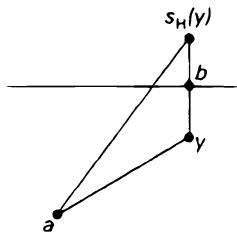
\includegraphics[keepaspectratio]{images/part001_5f5a2798.jpg}}\\
图 1

\begin{enumerate}
\def\labelenumi{(\roman{enumi})}
\setcounter{enumi}{1}
\item
设 \(\mathbf{C}'\) 是一个室且 \(a' \in \mathbf{C}'\)。由已证结果，存在 \(w \in \mathrm{W}_{\mathfrak{M}}\)，使得 \(w^{-1}(a') \in \overline{\mathbf{C}}\)；因此，室 \(\mathbf{C}'\) 与 \(\overline{w(\mathbf{C})}\) 相交；由于 \(\overline{w(\mathbf{C})}\) 是 \(w(\mathbf{C})\) 与内部为空的面片的并（《一般拓扑》第 §1 第 2 号命题 3），故 \(\mathbf{C}' = w(\mathbf{C})\)。
\item
我们必须证明 \(W = W_{\mathfrak{M}}\)，为此只需证明 \(s_{H'} \in W_{\mathfrak{M}}\) 对所有 \(H' \in \mathfrak{H}\) 成立。现在，\(H'\) 至少是一个室 \(C'\) 的墙（《一般拓扑》第 §1 第 4 号命题 8）；我们已经看到，存在 \(w \in W_{\mathfrak{M}}\) 使 \(C' = w(C)\)；于是存在一个墙 \(H\) 属于 \(C\)，使 \(H' = w(H)\)，从而 \(s_{H'} = w.s_H.w^{-1} \in W_{\mathfrak{M}}\)。
\end{enumerate}

\subsection{与 Coxeter 系统的关系}

定理 1. 设 \(\mathbf{C}\) 是一个室，令 \(\mathbf{S}\) 为关于 \(\mathbf{C}\) 的墙的反射所成的集合。

\begin{enumerate}
\def\labelenumi{(\roman{enumi})}
\item
有序对 \((\mathbf{W},\mathbf{S})\) 是一个 Coxeter 系统。
\item
设 \(w \in \mathrm{W}\)，且 \(\mathrm{H}\) 是 \(\mathrm{C}\) 的墙。关系 \(l(s_{\mathrm{H}}w) > l(w)\) 蕴含室 \(\mathrm{C}\) 与 \(w(\mathrm{C})\) 位于 \(\mathrm{H}\) 的同一侧。
\item
对于任意室 \(\mathbf{C}'\)，存在唯一的 \(w \in \mathbf{W}\)，使得 \(w(\mathbf{C}) = \mathbf{C}'\)。
\item
满足 \(\mathbf{H}\) 的超平面 \(s_{\mathrm{H}} \in \mathbf{W}\) 的集合等于 \(\mathfrak{H}\)。
\end{enumerate}

S 的每个元素的阶都是 2，而引理 2 表明 S 生成 W。对于 C 的任一墙 H，记 \(P_{H}\) 为满足下列条件的 \(w \in W\) 所成的集合：室 C 与 \(w(\mathrm{C})\)（它们不与 H 相交）位于 H 的同一侧。我们将验证《代数》第 IV 章 §1 第 7 号的 \((\mathrm{A}')\)、\((\mathrm{B}')\) 和 (C) 条件。

\((A') 1 \in P_H\)：显然。

(B') \(P_{H}\) 与 \(s_{H}.P_{H}\) 不相交：事实上，\(w(\mathrm{C})\) 和 \(s_{H}w(\mathrm{C})\) 位于 H 的相反两侧；因此，若 \(w(\mathrm{C})\) 与 C 在 H 的同一侧，它就不会与 \(s_{\mathrm{H}}w(\mathrm{C})\) 在同一侧。

\begin{enumerate}
\def\labelenumi{(\Alph{enumi})}
\setcounter{enumi}{2}
\tightlist
\item
设 \(w \in \mathrm{P_H}\)，且 \(\mathrm{H}'\) 是 \(\mathbf{C}\) 的一面墙，使 \(ws_{\mathrm{H}'} \notin \mathrm{P_H}\)；则 \(ws_{\mathrm{H}'} = s_{\mathrm{H}}w\)：根据假设，\(w(\mathbf{C})\) 与 \(\mathbf{H}\) 在 \(\mathbf{C}\) 的同一侧，而 \(ws_{\mathrm{H}'}(\mathbf{C})\) 在另一侧。因此，\(ws_{\mathrm{H}'}(\mathbf{C})\) 与 \(w(\mathbf{C})\) 位于 H 的相反两侧；所以，\(s_{\mathrm{H}^{\prime}}(\mathrm{C})\) 与 C 位于超平面 \(w^{-1}(\mathrm{H})\) 的相反两侧。令 a 为支撑为 \(H^{\prime}\) 的 C 的一个面上的点。点 \(a = s_{\mathrm{H}^{\prime}}(a)\) 同时属于室 C 与 \(s_{\mathrm{H}^{\prime}}(\mathrm{C})\) 的闭包，而这两个室分别包含于 \(w^{-1}(\mathrm{H})\) 所界定的两个开半空间中；于是 \(a \in w^{-1}(\mathrm{H})\)，故 \(\mathrm{H}^{\prime} = w^{-1}(\mathrm{H})\)。由此推出 \(s_{\mathrm{H}^{\prime}} = w^{-1}s_{\mathrm{H}}w\)，从而 \(ws_{H^{\prime}} = s_{H}w\)。
\end{enumerate}

断言 (i) 和 (ii) 由此以及《代数》第 IV 章 §1 第 7 号命题 6 得出。此外，我们有（同上，条件 (A)）

\[
\bigcap_ {H \in \mathfrak {M}} P _ {H} = \{1 \}.\tag{3}
\]

引理 2 表明 W 在室的集合上传递。此外，若 \(w \in W\) 满足 \(w(\mathrm{C}) = \mathrm{C}\)，则对 C 的每一面墙 H 都有 \(w \in P_{H}\)，因而由 (3) 得 w = 1。这证明了 (iii)。

最后，设 H 是满足 \(s_{H} \in W\) 的一个超平面。如果 H 不属于 H，则至少存在一个与 H 相交的室 \(C'\)（\(\S1\)，第 3 号命题 7）。\(H \cap C'\) 中的每个交点都在 \(s_{H}\) 作用下不变，因而同时属于室 \(C'\) 和 \(s_{\mathrm{H}}(\mathrm{C}')\)；所以，\(\mathrm{C}' = s_{\mathrm{H}}(\mathrm{C}')\)，这与 (iii) 矛盾，因为 \(s_{H} \neq 1\)。

推论. 设 \(\Sigma\) 是生成 W 的一组反射。那么属于 W 的每个反射都与 \(\Sigma\) 中的一个元素共轭。

令 \(\mathfrak{H}'\) 为形如 \(w(\mathrm{H})\) 的超平面所成的集合，其中 \(w \in \mathrm{W}\)、\(\mathrm{H} \in \mathfrak{H}\)，且 \(s_{\mathrm{H}} \in \Sigma\)。由于 \(\mathrm{W}\) 由族 \((s_{\mathrm{H}})_{\mathrm{H} \in \mathfrak{H}'}\) 生成，且 \(\mathfrak{H}'\) 在 \(\mathrm{W}\) 下稳定，我们可以用 \(\mathfrak{H}'\) 代替 \(\mathfrak{H}\) 应用本号的全部结果；但是定理 1(iv) 表明 \(\mathrm{W}\) 中的每个反射都形如 \(s_{\mathrm{H}}\)，其中 \(\mathrm{H} \in \mathfrak{H}'\)，因此推论得证。

\subsection{基本域与稳定子群}

回顾《积分》第 VII 章 §2 第 10 号定义 2：若 E 的子集 D 使 W 在 E 中的每个轨道都恰好与 D 相交于一点，则称 D 是群 W 的基本域。这等价于下列两个条件：

\begin{enumerate}
\def\labelenumi{\alph{enumi})}
\item
对于每个 \(x \in \mathrm{E}\)，存在 \(w \in \mathrm{W}\)，使得 \(w(x) \in \mathrm{D}\)。
\item
若 \(x, y \in D\) 且 \(w \in W\) 满足 \(y = w(x)\)，则 y = x（即使 \(w \neq 1\)）。
\end{enumerate}

我们将证明下列三个命题：

定理 2. 对任意室 C，C 的闭包 \(\overline{\mathbf{C}}\) 是 W 在 E 上作用的一个基本域。

命题 1. 设 \(\mathbf{F}\) 是一个面片，\(\mathbf{C}\) 是满足 \(\mathbf{F} \subset \overline{\mathbf{C}}\) 的室。设 \(w \in W\)。下列条件等价：

\begin{enumerate}
\def\labelenumi{(\roman{enumi})}
\item
\(w(\mathbf{F})\) 与 F 相交；
\item
\(w(\mathbf{F}) = \mathbf{F};\)
\item
\(w(\overline{\mathrm{F}}) = \overline{\mathrm{F}};\)
\item
w 至少固定 F 中的一个点；
\item
w 固定 F 的每一个点；
\item
w 固定 \(\overline{\mathbf{F}}\) 的每一个点；
\item
w 属于 W 中由包含 F 的 C 的墙的反射生成的子群。
\end{enumerate}

对于 E 的每个子集 A，记 \(W(A)\) 为 W 中由固定 A 的每一个点的元素所成的子群。

命题 2. 设 A 是 E 的非空子集，令 \(\mathfrak{H}_{\mathrm{A}}\) 为包含 A 的超平面 \(\mathrm{H} \in \mathfrak{H}\) 所成的集合，令 \(\mathrm{A}'\) 为这些 \(\mathrm{H} \in \mathfrak{H}_{\mathrm{A}}\) 的交，并令 F 为 E 中在 \(\mathrm{A}'\) 内部开着的一个面片（§1，第 3 号，命题 7）。则 \(\mathrm{W(A)} = \mathrm{W(A')} = \mathrm{W(F)}\)，且 \(\mathrm{W(A)}\) 由关于 \(\mathfrak{H}_{\mathrm{A}}\) 中超平面的反射生成。

我们先证明下列断言：

\begin{enumerate}
\def\labelenumi{(\Roman{enumi})}
\tightlist
\item
设 C 是一个室，设 x 和 y 是 \(\overline{C}\) 中的两个点，并设 \(w \in W\) 满足 \(w(x) = y\)。则 x = y，且 w 属于子群 \(W_{N}\)，其中 N 是包含 x 的 C 的墙的集合。
\end{enumerate}

我们对长度 \(q\) 的 \(w\)（相对于集合 \(S\)（由关于 \(C\) 的墙的反射组成））作归纳，\(q = 0\) 时结论显然。若 \(q \geqslant 1\)，则存在 \(H\) 为 \(C\) 的一个墙以及元素 \(w' \in W\)，使得 \(w = s_H w'\) 且 \(l(w') = q - 1\)。由于 \(l(s_H w) < l(w)\)，根据第 2 号的定理 1，室 \(C\) 与 \(w(C)\) 位于 \(H\) 的相反两侧。因此，\(\overline{C} \cap w(\overline{C}) \subset H\)，所以 \(y \in H\)。于是 \(y = w'(x)\)，归纳假设推出 \(x = y\) 且 \(w' \in W_{\mathfrak{N}}\)。由于 \(y \in H\)，可知 \(H \in \mathfrak{N}\)，从而 \(w = s_H w' \in W_{\mathfrak{N}}\)，(I) 的证明完成。

定理 2 的证明：这由 (I) 和引理 2 得出。

命题 1 的证明：我们知道两个不同的面片不相交且闭包不同（§1，第 2 号，命题 3 的推论）。因此 (i)、(ii)、(iii) 等价。另一方面，显然

\[
(\mathrm{vii}) \Longrightarrow (\mathrm{vi}) \Longrightarrow (\mathrm{v}) \Longrightarrow (\mathrm{iv}) \Longrightarrow (\mathrm{i})
\]

且断言 (I) 表明 (i) \(\Longrightarrow\) (vii)。

命题 2 的证明：令 \(\mathbf{A}''\) 为由 A 生成的 \(\mathbf{E}\) 的仿射子空间。显然，\(\mathrm{W(A)} = \mathrm{W(A'')}\)。由 §1 第 3 号的命题 7，存在点 \(x \in \mathbf{A}''\)，它不属于任何超平面 \(\mathbf{H} \in \mathfrak{H} - \mathfrak{H}_{\mathbf{A}}\)。令 \(\mathbf{F}_x\) 为包含 \(x\) 的面片：它在 \(\mathbf{A}''\) 中是开的，而命题 1 表明

\[
\mathrm{W} \left(\mathrm{F} _ {x}\right) \subset \mathrm{W} \left(\mathrm{A} ^ {\prime}\right) \subset \mathrm{W} (\mathrm{A}) = \mathrm{W} \left(\mathrm{A} ^ {\prime \prime}\right) \subset \mathrm{W} (\{x \}) = \mathrm{W} \left(\mathrm{F} _ {x}\right),
\]

从而 \(\mathrm{W(A) = W(A') = W(F_x)}\)。将 A 替换为 F，我们也有

\[
\mathrm{W} (\mathrm{A}) = \mathrm{W} (\mathrm{F}),
\]

因此命题得证。

注. 1) 由定理 2 可知，若 C 是一个室而 F 是一个面片，则存在唯一的面片 \(F'\) 包含于 \(\overline{C}\)，它被 W 的一个元素变换为 F。

\begin{enumerate}
\def\labelenumi{\arabic{enumi})}
\setcounter{enumi}{1}
\item
由命题 1 和 2 可知，对于 E 的任意非空子集 A，存在一点 \(a \in E\)，使得 \(W(A) = W(\{a\})\)；此外，群 \(W(A)\) 是一个 Coxeter 群（定理 1）。
\item
设 \(\mathbf{C}\) 是 \(\mathbf{E}\) 的一个室，\(\mathbf{S}\) 是关于 \(\mathbf{C}\) 的墙的反射所成的集合。设 \(w \in W\)，并设 \((s_1, \ldots, s_q)\) 是 \(w\) 关于 \(\mathbf{S}\) 的一个约化分解。若 \(x \in \overline{\mathbf{C}}\) 被 \(w\) 固定，则有 \(s_j(x) = x\) 对所有 \(j\) 成立：这由上述命题 1 以及《代数》第 IV 章 §1 的命题 7 的推论 1 得出。
\end{enumerate}

\subsection{W 的 Coxeter 矩阵与 Coxeter 图}

设 C 是一个室，\(S = S(C)\) 为关于 C 的墙的正交反射所成的集合，\(M = (m(s, s'))\) 为 Coxeter 系统 (W, S) 的 Coxeter 矩阵（《代数》第 IV 章 §1 第 9 号）；回顾 \(m(s, s')\) 是 W 中元素 \(ss'\) 的阶（有限或无限）（其中 \(s, s' \in S\)）。若 \(C'\) 是另一个室，则满足 \(w \in W\) 且 \(w(C) = C'\) 的唯一元素 w 定义一个双射

\[
s \mapsto f (s) = w s w ^ {- 1}
\]

从 S 到 \(S' = S(C')\)，并且有 \(m(f(s), f(s')) = m(s, s')\)。由此，如果 W 通过 \((C, s)\) 作用于由二元组 \(s \in S(C)\) 构成的集合 X，其中 C 是一个室且 \(w.(C, s) = (w(C), wsw^{-1})\)，则 W 在 X 中的每个轨道都与集合 \(\{C\} \times S(C)\) 恰好相交于一点，我们记该点为 \((C, s_i(C))\)。因此，若 I 是轨道集且 \(i, j \in I\)，数值 \(m_{ij} = m(s_i(C), s_j(C))\) 与室 C 的选择无关。矩阵 \(M(W) = (m_{ij})_{i,j \in I}\) 是一个 Coxeter 矩阵，称为 W 的 Coxeter 矩阵。与 M(W) 相关的 Coxeter 图（《代数》第 IV 章 §1 第 9 号）称为 W 的 Coxeter 图。

设 C 是一个室。对于任意 \(i \in I\)，记 \(\mathrm{H}_{i}(\mathrm{C})\) 为 C 的满足下述条件的墙：\(s_{i}(\mathrm{C})\) 是关于 \(\mathrm{H}_{i}(\mathrm{C})\) 的反射；并记 \(e_{i}(\mathrm{C})\) 为与 \(\mathrm{H}_{i}(\mathrm{C})\) 正交、且位于 \(\mathrm{H}_{i}(\mathrm{C})\) 与 C 同一侧的单位向量。映射 \(i \mapsto \mathrm{H}_{i}(\mathrm{C})\) 称为 C 的规范编号墙族。

命题 3. 设 \(\mathbf{C}\) 是一个室，且 \(i, j \in \mathbf{I}\) 满足 \(i \neq j\)。置 \(s_i = s_i(\mathbf{C})\)、\(\mathbf{H}_i = \mathbf{H}_i(\mathbf{C})\)、\(e_i = e_i(\mathbf{C})\)，并类似地定义 \(s_j\)、\(\mathbf{H}_j\) 和 \(e_j\)。

\begin{enumerate}
\def\labelenumi{(\roman{enumi})}
\item
若 \(\mathrm{H}_i\) 与 \(\mathrm{H}_j\) 平行，则 \(m_{ij} = \infty\) 且 \(e_i = -e_j\)。
\item
若 \(\mathrm{H}_i\) 与 \(\mathrm{H}_j\) 不平行，则 \(m_{ij}\) 有限，且
\end{enumerate}

\[
\left(e _ {i} \mid e _ {j}\right) = - \cos (\pi / m _ {i j}).\tag{4}
\]

\begin{enumerate}
\def\labelenumi{(\roman{enumi})}
\setcounter{enumi}{2}
\tightlist
\item
有 \((e_i|e_j)\leqslant 0\)。
\end{enumerate}

若 \(\mathrm{H}_i\) 与 \(\mathrm{H}_j\) 平行，则 \(s_i s_j\) 是一个平移（§2，第 4 号，命题 5），所以 \(m_{ij} = \infty\)。此外，或者 \(e_i = e_j\)，或者 \(e_i = -e_j\)。现在，闭包 C 中存在一点 \(a\)（分别为 \(a'\)），它属于 \(\mathrm{H}_i\)（分别属于 \(\mathrm{H}_j\)），但不属于 \(\mathrm{H}_j\) \((\text{resp. } \mathrm{H}_i)\)。于是 \((a' - a|e_i) > 0\) 且 \((a - a'|e_j) > 0\)，这排除了 \(e_i = e_j\) 的情形，并证明了 (i)。

现在假设 \(H_{i}\) 与 \(H_{j}\) 不平行。取 \(a \in H_{i} \cap H_{j}\) 为原点，并通过双射 \(t \mapsto a + t\) 将 T 与 E 识别。令 V 为与 \(H_{i} \cap H_{j}\) 正交且经过 a 的平面。置 \(\Gamma = V \cap D_{H_{i}}(C) \cap D_{H_{j}}(C)\)（其中 \(D_{H}(C)\) 表示由 H 界定且包含 C 的开半空间（§1，第 1 号）），并令 D（分别为 \(D'\)）为 V 中包含于 \(H_{i} \cap V\)（分别为 \(H_{j} \cap V\)）且包含于 \(\Gamma\) 闭包中的半直线。对 V 取适当的定向后，集合 \(\Gamma\) 是 V 中满足下式的开半直线 \(\Delta\) 的并：

\[
0 <   (\widehat {\mathrm{D} , \Delta}) <   (\widehat {\mathrm{D} , \mathrm{D} ^ {\prime}}).
\]

令 \(W'\) 为由 \(W\) 和 \(s_i\) 生成的 \(s_j\) 的子群。对于任意 \(w \in W'\)，超平面 \(w(H_i)\) 和 \(w(H_j)\) 属于 \(\mathfrak{H}\)，包含 \(H_i \cap H_j\)，且不与 C 相交。因此，它们不与 \(\Gamma\) 相交（§1，第 5 号，命题 10）。于是，§2 第 5 号命题 7 的推论蕴含 (ii)。

最后，断言 (iii) 直接由 (i) 和 (ii) 得出，因为 \(m_{ij} \geqslant 2\) 对 \(i \neq j\) 成立。

注. 公式 (4) 实际上对所有 \(i, j \in I\) 都成立：事实上，当 \(\pi / m_{ij} = 0\) 时，\(m_{ij} = \infty\)，而当 \(i = j\) 时，\(m_{ij} = 1\) 且 \((e_i | e_j) = 1\)。

\subsection{标量积为负的向量系}

引理 3. 设 \(q\) 是实向量空间 \(V\) 上的一个正二次型，\(B\) 是与之关联的对称双线性型。设 \(a_1, \ldots, a_n\) 是 \(V\) 中满足 \(B(a_i, a_j) \leqslant 0\) 对 \(i \neq j\) 的元素。

\begin{enumerate}
\def\labelenumi{(\roman{enumi})}
\tightlist
\item
若 \(c_{1}, \ldots, c_{n}\) 是满足 \(q\left(\sum_{i} c_{i} a_{i}\right) = 0\) 的实数，则
\end{enumerate}

\[
q \left(\sum_ {i} | c _ {i} | a _ {i}\right) = 0.
\]

\begin{enumerate}
\def\labelenumi{(\roman{enumi})}
\setcounter{enumi}{1}
\tightlist
\item
若 \(q\) 非退化，且存在 \(f\) 上的线性形式 \(V\)，使得 \(f(a_i) > 0\) 对所有 \(i\) 成立，则向量 \(a_1, \ldots, a_n\) 线性无关。
\end{enumerate}

关系 \(\mathrm{B}(a_i, a_j) \leqslant 0\) 对 \(i \neq j\) 立即推出

\[
q \left(\sum_ {i} | c _ {i} | a _ {i}\right) \leqslant q \left(\sum_ {i} c _ {i} a _ {i}\right),
\]

若 \(q\) 非退化，则关系 \(\sum_{i} c_{i} a_{i} = 0\) 从而蕴含

\[
\sum_ {i} | c _ {i} | a _ {i} = 0;
\]

于是，对于 \(f\) 上的任意线性形式 \(\mathbf{V}\)，有 \(\sum_{i}|c_i|f(a_i) = 0\)，从而 \(c_i = 0\) 对所有 \(i\) 成立，条件是还对所有 \(f(a_i) > 0\) 有 \(i\)。这证明了 (ii)。

引理 4. 设 \(\mathbf{Q} = (q_{ij})\) 是一个实的、对称的、\(n\) 阶方阵，满足：

\begin{enumerate}
\def\labelenumi{\alph{enumi})}
\item
  \(q_{ij} \leqslant 0\) for \(i \neq j\) ;
\item
不存在将 \(\{1,2,\ldots,n\}\) 划分为两个非空子集 I 和 J 的划分，使得 \((i,j)\in\mathrm{I}\times\mathrm{J}\) 蕴含 \(q_{ij}=0\)；
\item
二次型 \(q(x_{1},\ldots ,x_{n}) = \sum_{i,j}q_{ij}x_{i}x_{j}\) 定义在 \(\mathbf{R}^n\) 上且为正。
\end{enumerate}

于是：

\begin{enumerate}
\def\labelenumi{(\roman{enumi})}
\item
\(\mathbf{N}\) 是 \(q\) 的核，其维数为 0 或 1。若 \(\dim \mathbf{N} = 1\)，则 \(\mathbf{N}\) 由一个所有坐标均 \(> 0\) 的向量生成。
\item
\(\mathbf{Q}\) 的最小特征值的重数为 1，并且相应的特征向量的所有坐标均 \(>0\) 或均 \(< 0\)。
\end{enumerate}

由于 \(q\) 是正二次型，\(N\) 是 \(q\) 的迷向向量集合（关于 \(q\) 而言）（《代数》第 IX 章 §7 第 1 号命题 2 的推论）。令 \(a_1, \ldots, a_n\) 为 \(\mathbf{R}^n\) 的标准基。若 \(\sum_{i} c_i a_i \in N\)，引理 3 表明 \(\sum_{i} |c_i| a_i \in N\) 也成立，从而有 \(\sum_{i} q_{ji}|c_i| = 0\) 对所有 \(j\) 成立。令 \(I\) 为 \(i\) 满足 \(c_i \neq 0\) 时的指标集合。若 \(j \notin I\)，则 \(q_{ji}|c_i| \leqslant 0\) 对 \(i \in I\) 成立，而 \(q_{ji}|c_i| = 0\) 对 \(i \notin I\) 成立，所以 \(q_{ji} = 0\) 对 \(j \notin I\) 且 \(i \in I\) 成立。因此，假设 \(b)\) 蕴含 \(I = \varnothing\) 或 \(I = \{1, \ldots, n\}\)。于是，\(N\) 中每个非零向量的所有坐标都 \(\neq 0\)。若 \(\dim N \geqslant 2\)，则 \(N\) 与方程为 \(x_i = 0\) 的超平面的交的维数将 \(\geqslant 1\)，这与我们刚才证明的事实矛盾。前面的论证还表明，若 \(\dim N = 1\)，则 \(N\) 含有一个所有坐标均 \(>0\) 的向量。这证明了 (i)。

另一方面，我们知道 Q 的特征值为实数（《代数》第 IX 章 §7 第 3 号命题 5），且由于 q 为正的而为正。令 \(\lambda\) 为其中最小者。矩阵 \(Q' = Q - \lambda I_n\) 是退化正型 \(q'\) 的矩阵，而 \(Q'\) 的非对角元素与 Q 的相同。因此，\(Q'\) 满足本引理陈述中的条件 a)、b) 和 c)。由于 \(N'\) 是 \(q'\) 的核，且是 Q 对应于特征值 \(\lambda\) 的特征子空间，断言 (ii) 由 (i) 得出。

引理 5. 设 \(e_1, \ldots, e_n\) 是生成 \(T\) 的向量，满足：

\(a) (e_i | e_j) \leqslant 0 \text{ 当 } i \neq j;\)

\begin{enumerate}
\def\labelenumi{\alph{enumi})}
\setcounter{enumi}{1}
\tightlist
\item
不存在将 \(\{1, \ldots, n\}\) 划分为两个非空子集 I 和 J 的划分，使得 \((e_i|e_j) = 0\) 对 \(i \in I\) 且 \(j \in J\) 成立。
\end{enumerate}

于是有两种可能：

\begin{enumerate}
\def\labelenumi{\arabic{enumi})}
\item
\((e_1, \ldots, e_n)\) 是 T 的一个基；
\item
\(n = \dim T + 1\)；存在一个族 \((c_i)_{1 \leqslant i \leqslant n}\)，其元素为 \(> 0\) 的实数，并满足 \(\sum_{i} c_i e_i = 0\)，并且任何实数族 \((c_i')_{1 \leqslant i \leqslant n}\) 满足 \(\sum_{i} c_i' e_i = 0\) 时，都与 \((c_i)_{1 \leqslant i \leqslant n}\) 成比例。
\end{enumerate}

置 \(q_{ij} = (e_i|e_j)\)。于是矩阵 \(Q = (q_{ij})\) 满足引理 4 的假设：引理 4 的条件 a) 和 b) 分别就是上述条件 a) 和 b)，而 c) 得到满足，因为 \(\sum_{i,j} q_{ij} x_i x_j = \|\sum_{i} x_i e_i\|^2\)。\(q\) 在 \(\mathbf{R}^n\) 上且矩阵为 \(\mathbf{Q}\) 的二次型的核 N，是 \((c_1, \ldots, c_n) \in \mathbf{R}^n\) 中满足 \(\sum_{i} c_i e_i = 0\) 的向量所成的集合。若 \(N = \{0\}\)，则 \(e_i\) 线性相关，我们处于情形 1)。若 \(\dim N > 0\)，引理 4(i) 表明我们处于情形 2)。

引理 6. 设 \((e_1, \ldots, e_n)\) 是 T 的一个基，且 \((e_i | e_j) \leqslant 0\) 对 \(i \neq j\) 成立。

\begin{enumerate}
\def\labelenumi{(\roman{enumi})}
\item
若 \(x = \sum_{i} c_i e_i \in \mathbf{T}\) 满足 \((x|e_i) \geqslant 0\) 对所有 \(i\) 成立，则 \(c_i \geqslant 0\) 对所有 \(i\) 成立。
\item
若 \(x\) 和 \(y\) 是 \(\mathrm{T}\) 中的两个元素，满足 \((x|e_i) \geqslant 0\) 且 \((y|e_i) \geqslant 0\) 对所有 \(i\) 成立，则 \((x|y) \geqslant 0\)。若 \((x|e_i) > 0\) 且 \((y|e_i) > 0\) 对所有 \(i\) 成立，则 \((x|y) > 0\)。
\end{enumerate}

在 (i) 的假设下，假设某个 \(c_{i} < 0\)，其中 \(i\) 为固定指标。令 \(f\) 为 \(T\) 上由 \(f(e_{i}) = 1\) 定义的线性形式，并且

\[
f \left(e _ {j}\right) = - c _ {i} / \left(\sum_ {k = 1} ^ {n} \left| c _ {k} \right|\right) \quad \text { for } j \neq i.
\]

于是，向量 \(-x, e_1, \ldots, e_n\) 满足引理 3(ii) 的假设（取 T 上的度量型作为 \(q\)）。我们得到它们线性无关，这不可能。因此 (i) 成立。此外，若 \(x = \sum_{i} c_i e_i \in \mathbf{T}\) 且 \(y \in \mathbf{T}\)，则 \((x|y) = \sum_{i} c_i (e_i | y)\)，所以 (ii) 立即由 (i) 得出。

\subsection{有限性定理}

引理 7. 设 A 是 T 中的单位向量集。若存在实数 \(\lambda < 1\)，使得 \((a|a') \leqslant \lambda\) 对于 \(a, a' \in \mathbf{A}\) 且 \(a \neq a'\) 成立，则 A 是有限集。

对于 \(a, a' \in A\) 且 \(a \neq a'\)，有

\[
\left\| a - a ^ {\prime} \right\| ^ {2} = 2 - 2 (a \mid a ^ {\prime}) \geqslant 2 - 2 \lambda .
\]

现在，T 的单位球面 S 是紧的，因此存在一个由直径 \(<(2-2\lambda)^{1/2}\) 的集合组成的有限覆盖，并且这些集合中每个至多包含 A 的一个点，于是引理得证。

记 \(U(w)\) 为与从 E 到自身的仿射映射 \(w \in W\) 相关联的 T 的自同构。我们有

\[
w (x + t) = w (x) + \operatorname{U} (w). t \text {for} t \in \mathrm{T} \text {and} x \in \mathrm{E}.
\]

这定义了从群 W 到 T 的正交群的同态 U；U 的核是属于 W 的平移。

定理 3. (i) 一个室的墙的集合是有限的。

\begin{enumerate}
\def\labelenumi{(\roman{enumi})}
\setcounter{enumi}{1}
\item
属于 \(\mathfrak{H}\) 的超平面的方向的集合是有限的。
\item
群 U(W) 是有限的。
\end{enumerate}

断言 (i) 立即由命题 3(iii) 和引理 7 得出。

设 \(\mathbf{C}\) 是一个室，\(\mathfrak{M}\) 是其墙的集合。\(\overline{\mathbf{C}}\) 的面片（相对于 \(\mathfrak{H}\)）与相对于 \(\mathfrak{M}\) 的相同（§ 1，第 4 号，命题 9）。

由于 M 是有限的，面片的数目也是有限的。由于一个面片只与有限个属于 H 的超平面相交，所以与 \(\overline{C}\) 相交的属于 H 的超平面集合是有限的，因而 A(C)（即与某个属于 H 且与 \(\overline{C}\) 相交的超平面正交的 T 中单位向量的集合）也是有限的。因此，存在实数 \(\lambda < 1\)，使得 \((a|a') \leqslant \lambda\) 对于 \(a, a' \in A(C)\) 且 \(a \neq a'\) 成立。

令 A 为与属于 H 的某个超平面正交的 T 中单位向量所成的集合。设 \(a, a' \in A\) 且 \(a \neq a'\)。若 a 与 \(a'\) 平行，则 \(a = -a'\) 且 \((a|a') = -1\)。否则，令 \(H \in H\)（分别为 \(H' \in H\)）满足 a（分别为 \(a'\)）与 H（分别与 \(H'\)）正交。我们有 \(H \cap H' \neq \varnothing\)，且若 \(x \in H \cap H'\)，则存在元素 \(w \in W\)，使得 \(x \in w(\overline{C})\)。于是，向量 \(U(w).a\) 和 \(U(w).a'\) 属于 A(C)，且有

\[
(a \mid a ^ {\prime}) = (\mathrm{U} (w). a \mid \mathrm{U} (w). a ^ {\prime}) \leqslant \lambda ,
\]

且由引理 7，集合 \(\mathbf{A}\) 是有限的。因此 (ii)。

现在，设 \(w \in W\)，满足 \(\mathrm{U}(w).a = a\) 对所有 \(a \in A\) 成立。则 \(\mathrm{U}(w).t = t\) 对 T 中由 A 生成的子空间内的所有 t 成立。另一方面，若 \(t \in T\) 与 A 正交，则对所有 \(\mathrm{U}(s_{\mathrm{H}}).t = t\) 都有 \(H \in H\)，因而 \(\mathrm{U}(w).t = t\)，最终 \(\mathrm{U}(w) = 1\)。由于对所有 \(\mathrm{U}(w)(\mathrm{A}) = \mathrm{A}\) 都有 \(w \in W\)，我们得到 \(\mathrm{U}(\mathrm{W})\) 同构于有限集 A 的一个置换群，因此 (iii)。

命题 4. 设 C 是一个室，N 是 C 的一组墙。令 \(W_{N}\) 为由关于 N 中元素的正交反射生成的 W 的子群。对于 \(H \in N\)，记 \(e_{H}\) 为与 H 正交且位于 H 与 C 同一侧的单位向量。下列条件等价：

\begin{enumerate}
\def\labelenumi{(\roman{enumi})}
\item
群 \(\mathbf{W}_{\mathfrak{N}}\) 是有限的。
\item
存在 \(\mathbf{E}\) 中一点，在 \(W_{\mathfrak{N}}\) 的每个元素下不变。
\item
属于 \(\mathfrak{N}\) 的超平面有非空交。
\item
向量族 \((e_{\mathrm{H}})_{\mathrm{H}\in \mathfrak{N}}\) 在 T 中自由。
\end{enumerate}

根据 §3 开头的性质 (D2)，W 中每一点的稳定子都是有限的，因此 (ii) 蕴含 (i)。

由于群 \(W_{N}\) 由关于属于 N 的超平面所成的反射集合生成，\(W_{N}\) 的不动点就是属于每个超平面 \(H \in N\) 的 E 中的点，因此 (ii) 与 (iii) 等价。

假设 \(a\) 是 \(E\) 中的一点，使得 \(a \in H\) 对所有 \(H \in \mathfrak{N}\) 成立，并令 \(t \in T\) 满足 \(a + t \in C\)。由于 \((e_H | e_{H'}) \leqslant 0\) 对满足 \(H, H' \in \mathfrak{N}\) 且 \(H \neq H'\) 的情形成立（命题 3），又由于 \((t | e_H) > 0\) 对所有 \(H \in \mathfrak{N}\) 成立，引理 3(ii) 蕴含 \(e_H\)（其中 \(H \in \mathfrak{N}\)）线性无关。因此，(iii) 蕴含 (iv)。

最后，假设向量族 \((e_{\mathrm{H}})_{\mathrm{H}\in\mathfrak{N}}\) 是自由的。令 a 为 E 中一点。对于任意 \(H\in N\)，存在实数 \(c_{H}\)，使得 H 恰好由 E 中满足 \(a+t\) 的点 \((t|e_{\mathrm{H}})=c_{\mathrm{H}}\) 组成。由于族 \((e_{\mathrm{H}})\) 是自由的，存在 \(t\in T\)，使得 \((t|e_{\mathrm{H}})=c_{\mathrm{H}}\) 对所有 \(H\in N\) 成立，且 E 中的点 \(a+t\) 属于所有超平面 \(H\in N\)。因此，(iv) 蕴含 (iii)。

注. 1) 由于 W 由关于室 C 的墙的反射生成，前一命题给出了 W 有限的一个判据。我们将在第 9 号回到这个问题。

\begin{enumerate}
\def\labelenumi{\arabic{enumi})}
\setcounter{enumi}{1}
\tightlist
\item
设 F 是有限维实仿射空间，G 是 F 的自同构群。对于所有 \(g \in G\)，记 \(U(g)\) 为与 g 相关的 F 的平移空间 V 的自同构。假设 \(U(G)\) 的像是 \(\mathbf{GL}(V)\) 的有限子群；则 V 具有一个在 \(U(G)\) 下不变的标量积（《积分》第 VII 章 §3 第 1 号命题 1）。此外，如果 G 配备离散拓扑后在 F 上适当地作用，且由反射生成，则可以将本段的结果应用于 G。
\end{enumerate}

\subsection{W 在 T 上的线性表示的分解}

令 I 为 W 的 Coxeter 图的顶点集（第 4 号），令 J 为 I 的一个子集，使 J 中没有顶点与 I-J 中的任何顶点相连。设 C 是一个室，s 是从 I 到关于 C 的墙的反射集合的规范双射，并令 \(W_{J,C}\) 为由像 \(s(\mathrm{J})\) 生成的子群。由《代数》第 IV 章 §1 第 9 号命题 8 可知，W 是两个子群 \(W_{J,C}\) 和 \(W_{I-J,C}\) 的直积。设 \(C'\) 是另一个室，\(s'\) 是从 I 到 W 的相应单射。我们已经看到（第 4 号），若 \(w \in W\) 将 C 变换为 \(C'\)，则有 \(s'(\mathrm{i}) = ws(\mathrm{i})w^{-1}\)，其中 \(i \in I\)。由于 \(W_{J,C}\) 在 W 中正规，可知 \(s'(\mathrm{i}) \in W_{J,C}\) 对所有 \(i \in J\) 成立。我们推得子群 \(W_{J,C}\) 与 C 无关。从现在起将其简记为 \(W_{J}\)。

\(W_{J,C}\) 的定义显然可推广到 I 的任意子集 J。但是，如果 J 中有一个顶点与 I-J 中的一个顶点相连，则 \(W_{J,C}\) 不正规并且取决于 C 的选择。

令 \(T_{J}^{0}\) 为 T 中在 \(U(W_{J})\) 的每个元素下不变的向量所成的子空间，令 \(T_{J}\) 为与 \(T_{J}^{0}\) 正交的子空间。由于 \(W_{J}\) 是 W 的正规子群，显然 \(T_{J}^{0}\) 在 \(U(W)\) 下不变，因而 \(T_{J}\) 也是如此。

命题 5. 设 \(J_{1},\ldots,J_{s}\) 是 W 的 Coxeter 图的连通分支的顶点集。对于 \(1\leqslant p\leqslant s\)，置

\[
\mathrm{W} _ {p} = \mathrm{W} _ {\mathrm{J} _ {p}}, \quad \mathrm{T} _ {p} = \mathrm{T} _ {\mathrm{J} _ {p}}; \quad \mathrm{T} _ {p} ^ {\prime} = \mathrm{T} _ {\mathrm{J} _ {p}} ^ {0}, \quad \text {and} \quad \mathrm{T} _ {0} = \bigcap_ {1 \leqslant p \leqslant s} \mathrm{T} _ {p} ^ {\prime}.
\]

\begin{enumerate}
\def\labelenumi{(\roman{enumi})}
\item
群 W 是群 \(\mathrm{W}_p\) 的直积（\(1 \leqslant p \leqslant s\)）。
\item
空间 \(\mathbf{T}\) 是子空间 \(\mathrm{T}_0, \mathrm{T}_1, \ldots, \mathrm{T}_s\) 的正交直和，它们都在 \(\mathrm{U}(\mathrm{W})\) 下稳定。
\item
对于所有 \(q\) 满足 \(1 \leqslant q \leqslant s\)，子空间 \(\mathrm{T}_q'\) 是 \(\mathrm{T}\) 中由在 \(\mathrm{U}(\mathrm{W}_q)\) 的每个元素下不变的向量所成的；它是 \(\mathrm{T}_p\)（\(1 \leqslant p \leqslant s\) 且 \(p \neq q\)）的直和。
\item
设 \(\mathbf{C}\) 是一个室。子空间 \(\mathrm{T}_p\)（\(1 \leqslant p \leqslant s\)）由向量 \(e_i(\mathbf{C})\)（其中 \(i \in \mathrm{J}_p\)）生成（按第 4 号的记号）。
\item
W 在子空间 \(T_{p}\)（\(1 \leqslant p \leqslant s\)）上的表示是绝对不可约、非平凡且两两不等价的。
\end{enumerate}

断言 (i) 由《代数》第 IV 章 §1 第 9 号得出。另一方面，我们已经看到子空间 \(\mathrm{T}_p\) 在 \(\mathrm{U}(\mathrm{W})\) 下不变，\(\mathrm{T}_0\) 也如此。设 \(\mathrm{C}\) 是一个室；由于 \(\mathrm{W}_p\) 由反射 \(s_i(\mathrm{C})\)（其中 \(i \in \mathrm{J}_p\)）生成，显然 \(\mathrm{T}_p'\) 是与 \(e_i(\mathrm{C})\)（其中 \(i \in \mathrm{J}_p\)）正交的子空间，因而得到 (iv)。此外，若 \(i \in \mathrm{J}_p\)、\(j \in \mathrm{J}_q\) 且 \(p \neq q\)，则 \(m_{ij} = 2\)，因为 \(\{i,j\}\) 不是 \(\mathrm{W}\) 的 Coxeter 图的一条边，所以 \((e_i|e_j) = 0\)。断言 (ii) 现已显然。断言 (iii) 则随之得出，因为 \(\mathrm{T}_q'\) 是 \(\mathrm{T}_q\) 的正交补。

最后，设 V 是在 \(T_{p}\) 下不变的 \(\mathrm{U}(\mathrm{W}_{p})\) 的子空间。对于所有 \(i \in J_{p}\)，要么 \(e_{i} \in V\)，要么 \(e_{i}\) 与 V 正交（\(\S2\)2，第 2 号，命题 3）。令 A（分别为 B）为满足 \(i \in J_{p}\)（分别为 \(e_{i} \in V\) 与 V 正交）的 \(e_{i}\) 所成的集合。显然，对 \((e_{i}|e_{j}) = 0\) 且 \(i \in A\) 有 \(j \in B\)，而由于 \(J_{p}\) 连通，可知或者 A = \(\varnothing\) 且 V = \(\{0\}\)，或者 A = \(J_{p}\) 且 V = \(T_{p}\)。因此，\(W_{p}\) 在 \(T_{p}\) 上的表示是不可约的，从而是绝对不可约的（\(\S2\)2，第 1 号，命题 1）。根据 \(T_{p}\) 的定义，它是非平凡的。最后，(v) 中的最后一个断言立即由 (iii) 得出。

如果 T 中在 U(W) 下不变的子空间 \(T_{0}\) 缩减为 \(\{0\}\)，则称 W 是本质的；如果 W 在 T 上的表示 U 是不可约的，则称 W 是不可约的。

推论. 假设 \(W \neq \{1\}\)。则 W 不可约，当且仅当它是本质的且其 Coxeter 图连通。

注. 在命题 5 的假设下，\(T_{p}\)（\(0 \leqslant p \leqslant s\)）是 W 在 T 上的线性表示 U 的等型分量（《代数》第 VIII 章 §3 第 4 号）。由此（同上，命题 11），T 中每个在 W 下稳定的向量子空间 V 都是 \(V \cap T_{p}\)（\(0 \leqslant p \leqslant s\)）之和；此外（同上，命题 10），每个与 \(U(w)\) 的算子 \(w \in W\) 对易的自同态都使每个 \(T_{p}\)（\(0 \leqslant p \leqslant s\)）保持稳定，并且对 \(1 \leqslant p \leqslant s\) 在其上诱导一个仿射伸缩。特别地，T 上在 W 下不变的双线性型 \(\Phi\) 是由下式给出的双线性型

\[
\varPhi \left(\sum_ {k} t _ {k}, \sum_ {k} t _ {k} ^ {\prime}\right) = \varPhi_ {0} (t _ {0}, t _ {0} ^ {\prime}) + \sum_ {1 \leqslant p \leqslant s} a _ {p} (t _ {p} | t _ {p} ^ {\prime}),
\]

其中 \(\Phi_{0}\) 是 \(T_{0}\) 上的双线性型，而 \(a_{p}\)（对 \(1 \leqslant p \leqslant s\)）是一个实数：事实上，这样的型 \(\Phi\) 可以唯一地写成 \((t, t') \mapsto (\mathrm{A}(t)|t')\) 的形式，其中 A 是一个与 \(\mathrm{U}(w)\) 的 \(w \in W\) 对易的 T 的自同态。
